\documentclass[12pt,a4paper]{article}
\usepackage[utf8]{inputenc}
\usepackage[russian]{babel}
\usepackage{indentfirst}
\usepackage{amsmath}
\usepackage{amsfonts}
\usepackage{amssymb}
\usepackage{graphicx}
\usepackage{float}
\usepackage[colorlinks=true,linkcolor=black,citecolor=black,urlcolor=blue]{hyperref}
\usepackage{geometry}
\geometry{a4paper, margin=2.5cm}
\pagestyle{plain}

\begin{document}

\begin{titlepage}
\centering

\vspace*{0cm}

ПРАВИТЕЛЬСТВО РОССИЙСКОЙ ФЕДЕРАЦИИ\\[0.3cm]
ФГАОУ ВО НАЦИОНАЛЬНЫЙ ИССЛЕДОВАТЕЛЬСКИЙ УНИВЕРСИТЕТ\\[0.2cm]
«ВЫСШАЯ ШКОЛА ЭКОНОМИКИ»\\[1cm]
Факультет компьютерных наук\\[0.2cm]
Образовательная программа «Прикладная математика и информатика»

\vspace{4cm}

\textbf{Отчет об исследовательском проекте на тему:}

\vspace{0.5cm}

\textbf{«Методы анализа временных рядов и обнаружения изменений»}

\vfill

\noindent
\begin{tabular}{@{}l}
\textbf{Выполнил:}\\[0.3cm]
студент группы БПМИ244\\
Крутиков Никита\\[1cm]
\textbf{Принял руководитель проекта:}\\[0.3cm]
Лукьянченко Петр Павлович\\
Заведующий проектно-учебной лабораторией\\
«Искусственный интеллект в математических финансах»
\end{tabular}

\vspace{2cm}

\centering
\textbf{Москва 2026}

\end{titlepage}

\newpage

\tableofcontents

\newpage

\section{Введение и постановка задачи}

Анализ временных рядов нередко предполагает обнаружение моментов, в которые статистические свойства данных претерпевают резкие изменения. Такие точки разладки (change points, CP) соответствуют смене состояния системы или внешних условий и могут существенно влиять на дальнейшее поведение ряда. Задача обнаружения разладок (change point detection  -- CPD) состоит в том, чтобы по наблюдаемому ряду выявить моменты, когда изменяется закон генерации данных. CPD применяется в задачах мониторинга физических процессов и финансовых систем. В обоих случаях динамику часто моделируют стохастическими дифференциальными уравнениями (SDE)  -- в физике как описание реального процесса, в финансах как приближение для ценообразования и управления рисками. В данной работе мы используем SDE с синусоидальным потенциалом -- модель из статистической физики. Ее математический аппарат (шум-индуцированные переходы между состояниями) переносится и на задачи смены режимов в финансовых рядах.

Есть два режима CPD. В офлайне весь ряд уже перед нами, и мы ищем разладки задним числом  -- это задача сегментации. В онлайне данные поступают в потоке, и нужно зафиксировать разладку как можно быстрее. Мы работаем в офлайне, хотя некоторые из наших методов (CUSUM) изначально создавались для потока.

\subsection{Актуальность проблемы}

В реальных данных изменения режима генерации сигнала могут указывать на важные события или структурные сдвиги в системе. Зная, где происходят разладки, можно анализировать каждый режим отдельно, а не усреднять по всему ряду. Прогнозные модели на однородных участках будут точнее. Без детекции точек разладки любая модель, построенная на <<склеенных>> режимах, рискует дать бессмысленный результат.

Для SDE-траекторий разладка проявляется как перескок процесса между устойчивыми состояниями  -- скачок уровня, который маскируется шумом и колебаниями вблизи границы между состояниями. Классические тесты предполагают один скачок среднего; нейросети могут выучить более сложный паттерн. Это определяет главный вопрос работы: выяснить, какой метод оптимален при каких параметрах. За десятилетия предложены десятки алгоритмов офлайн-CPD (обзор  -- в разделе~2), не считая онлайн-методов. У каждого свои предположения и своя ниша, а универсального решения нет. Отсюда мотивация: разобраться, что когда работает. Не абстрактно, а на конкретных данных с контролируемыми параметрами.

\subsection{Цель, новизна и задачи}

\textbf{Цель работы}  -- сравнить классические статистические и современные нейросетевые методы обнаружения точек разладки применительно к траекториям стохастических дифференциальных уравнений (SDE) и определить, какие подходы оптимальны в зависимости от параметров динамической системы.

В отличие от большинства бенчмарков CPD, где разладки создаются искусственно (скачок среднего, смена дисперсии), мы работаем с данными из нелинейной SDE вида $dx = \sin(x)\,dt + \sqrt{D}\,dW$, где $D$  -- коэффициент диффузии (интенсивность шума), $dW$  -- приращение винеровского процесса. Здесь разладки возникают сами  -- процесс проводит время вблизи устойчивых положений и иногда перескакивает между ними под действием шума. Такая постановка ближе к физическим задачам, где изменение режима  -- не внешнее вмешательство, а следствие динамики самой системы.

\textbf{Научная новизна} состоит в следующем:
\begin{enumerate}
    \item Впервые проведено систематическое сравнение широкого набора методов CPD разных классов  -- от ранговых тестов до Transformer  -- на траекториях нелинейной SDE, где разладки порождаются динамикой самого процесса, а не вставляются искусственно.
    \item Проведен статистический анализ переходов в SDE-процессе при разных уровнях шума и шагах дискретизации. Цель  -- понять, как параметры генерации влияют на структуру данных и какие методы детекции лучше подходят в каждом режиме.
    \item Впервые проведено экспериментальное исследование зависимости оптимального класса методов CPD от уровня шума в SDE-процессе с целью определить границу между режимами.
\end{enumerate}

\textbf{Задачи:}
\begin{enumerate}
    \item На основе модели из лаборатории научного руководителя (ноутбук с SDE-генератором и схемой Эйлера--Маруямы) реализовать воспроизводимый генератор траекторий с контролируемыми параметрами ($D$, $dt$, тип шума) и автоматической разметкой точек разладки.
    \item Реализовать и протестировать широкий набор методов CPD разных классов -- от ранговых тестов до нейросетей.
    \item Провести статистический анализ SDE-процесса: проверить гипотезы о распределении межпереходных расстояний, перелетов и числа разладок при варьировании параметров.
    \item Провести полный цикл экспериментов на 4 сценариях (разные $D$ и типы шума) с 50 тестовыми рядами на метод и строгим разделением обучение/калибровка/тест.
    \item Сформулировать практические рекомендации: какой класс методов применять в зависимости от характеристик данных.
\end{enumerate}

\section{Обзор литературы и мотивация}

\subsection{Общие сведения о CPD}

Первый формальный метод CPD  -- CUSUM  -- предложен Page~\cite{page1954} для контроля качества на производстве. С тех пор область разрослась: Truong et al.~\cite{truong2020} насчитали более 140 алгоритмов офлайн-CPD, разложив каждый на три блока: критерий однородности сегмента, процедура поиска разбиения и регуляризация числа разрывов. Их библиотека \texttt{ruptures} на Python стала стандартным инструментом. Aminikhanghahi и Cook~\cite{aminikhanghahi2017} дают более широкий обзор, включая онлайн-методы, и подчеркивают: CPD ищет момент смены закона генерации, а не просто выброс  -- это другая задача, нежели anomaly detection. Систематических сравнений на данных с нелинейной динамикой при этом нет.

\subsection{Категории методов}

Методы CPD принято делить на четыре класса, хотя границы условны. Для нашей задачи ключевые два.

Первый  -- \textbf{тесты на однородность}: проверяют, различаются ли параметры ряда до и после предполагаемой точки. Сюда входят ранговые критерии (Петтитт, Манн-Уитни), кумулятивные схемы (CUSUM) и тесты из климатологии (SNHT  -- Standard Normal Homogeneity Test, Буишанд). Большинство ищут одну точку за прогон  -- на рядах с десятками разладок это ограничение.

Второй  -- \textbf{методы скользящих окон}, сравнивающие поведение ряда <<до>> и <<после>> текущего момента по мерам различия между распределениями или отношению плотностей. Методы оценки отношения плотностей~\cite{liu2013} оценивают $p_{\text{after}}/p_{\text{before}}$ напрямую. Все наши ML-методы тоже работают в этой парадигме: CatBoost сравнивает статистики половин окна, нейросети обучаются различать <<окно с разладкой>> от <<окна без>>. Главная сложность на практике  -- выбор ширины окна.

Отдельно стоят \textbf{алгоритмы оптимальной сегментации} (PELT~\cite{killick2012}, MDL)  -- они разбивают ряд на однородные куски, штрафуя за лишние разладки. \textbf{Байесовские подходы} (BOCPD~\cite{adams2007}) дают вероятность разладки в каждой точке, но взамен требуют задать модель данных и априорное распределение длительности сегмента (функцию, задающую вероятность разладки в каждый момент при условии, что до сих пор её не было -- hazard function). Ещё один подход  -- автоэнкодеры (ALACPD~\cite{atashgahi2022}): они учатся восстанавливать нормальный сигнал, и разладку фиксируют по росту ошибки восстановления.

\subsection{Сравнительные исследования}

Прямых сравнений CPD-методов немного. Те что есть~\cite{truong2020, liu2013, hushchyn2020} проведены на кусочно-стационарных данных  -- когда ряд искусственно переключается между режимами  -- и приходят к одному выводу: лучший метод зависит от данных. При этом ни одно сравнение не проводилось на данных, где разладки возникают из динамики самой системы, а не вставляются вручную. Наша работа закрывает этот пробел.

\subsection{Что следует из обзора}

Обзор определяет три ключевых параметра эксперимента.

Методов много, и они очень разные. Необходимо охватить методы разных классов  -- от ранговых тестов до нейросетей,  -- чтобы не заузить сравнение. Ряд подходов (PELT, BOCPD, RuLSIF, Kernel CPD) сознательно оставлен за рамками: PELT превращает сравнение в подбор функции стоимости и штрафа, BOCPD требует задания hazard-функции, а RuLSIF и Kernel CPD концептуально близки к нашему CatBoost (сравнение окон <<до>> и <<после>>), но без обучения на данных. Метрик тоже хватает: одни работы смотрят на задержку обнаружения, другие  -- на precision/recall, третьи  -- на ROC-AUC. Мы используем шесть метрик параллельно, потому что ни одна из них в отдельности не дает полной картины.

Тестовые данные в литературе почти всегда кусочно-стационарные: ряд $\mathcal{N}(0,1)$, потом $\mathcal{N}(3,1)$, и вот вам changepoint. Это удобно, но далеко от реальных задач, где разладки порождаются динамикой самой системы, а не внешним переключением. Мы используем траектории SDE, в которых переходы между устойчивыми состояниями возникают естественно  -- и это, насколько нам известно, первое сравнение CPD-методов на таких данных.

Одна из центральных гипотез, вынесенных из обзора: нейросети должны побеждать на сложных паттернах, но проигрывать на простых. Эту гипотезу мы проверяем экспериментально в разделе~7.


\section{Обзор методов CPD}

\begin{enumerate}
    \item \textbf{CUSUM (Cumulative Sum)}  -- классический онлайн-метод Page~\cite{page1954}, накапливающий отклонения от ожидаемого среднего и срабатывающий при превышении порога. Единственный классический метод в нашем наборе, способный находить множественные CP: CUSUM последовательно обнаруживает десятки разладок, тогда как single-CP тесты (SNHT, Chow) находят одну. Расплата за высокий recall  -- ложные срабатывания: CUSUM реагирует на любой сдвиг среднего, в том числе вызванный шумом.

    \item \textbf{CatBoost (градиентный бустинг на признаках окна)}  -- из каждого окна длиной $W$ извлекаются 14 статистик (полный список  -- в \texttt{catboost\_cpd.py}), на которых обучается \texttt{CatBoostClassifier}. Ключевые четыре:

    \begin{tabular}{ll}
    $\bar{x}_L - \bar{x}_R$ & разность средних левой и правой половин окна \\
    $\sigma_L - \sigma_R$ & разность стандартных отклонений половин \\
    slope & наклон линейного тренда внутри окна \\
    $r_1$ & автокорреляция с лагом 1 \\
    \end{tabular}

    \smallskip
    Признаки $\bar{x}_L - \bar{x}_R$ и $\sigma_L - \sigma_R$  -- самые информативные: если в центре окна есть разладка, левая и правая половины будут различаться по уровню или разбросу. CatBoost быстро учится (минуты на CPU) и позволяет через оценку важности признаков (feature importance) увидеть, какие статистики <<ловят>> разладку. Главное ограничение -- фиксированный набор из 14 признаков. Если разладка проявляется через статистику, не вошедшую в набор, метод ее пропустит. Нейросети этого ограничения лишены. CatBoost не имеет v2-версии: при обучении на v2-данных ($D \in [0.2, 1.0]$, $W = 100$) результат улучшился незначительно, и мы оставили единственную конфигурацию ($W = 50$, 500 деревьев).
    
    \item \textbf{Рекуррентные нейросетевые подходы к CPD: LSTM и GRU}  -- класс методов, в которых задача детекции разладки формулируется как бинарная классификация скользящего окна рекуррентной сетью. В нашей реализации оба метода используют единую схему: окно фиксированной длины нормируется и подается на вход рекуррентной сети, которая по последнему скрытому состоянию предсказывает вероятность разладки в центре окна; модели обучаются на синтетических данных с разными типами шума и параметрами, после чего применяются к тестовому ряду поточечно, а конечное множество точек разладки извлекается через пороговую бинаризацию и подавление немаксимумов (NMS).

    \textit{LSTM (Long Short-Term Memory)} оснащен механизмом памяти ячейки (cell state) и тремя вентилями (входным, забывания и выходным), что позволяет явно управлять долгосрочной памятью и потенциально полезно для улавливания отложенных или постепенных разладок. Модель содержит больше параметров и требует существенно большего времени обучения.

    \textit{GRU (Gated Recurrent Unit)} упрощает LSTM до двух вентилей  -- сброса и обновления  -- без отдельного cell state. GRU имеет меньше параметров и обучается быстрее при сопоставимом качестве на контекстах средней длины. GRU включен как контрольное сравнение: если он покажет результат, близкий к LSTM, значит, дело в самой рекуррентности, а не в механизме cell state. У обоих методов общие слабости: им нужно много обучающих данных, и они могут переобучиться на конкретный тип шума. Кроме того, в отличие от классических тестов, у нейросетей нет формальных гарантий на долю ложных срабатываний  -- порог подбирается эмпирически.
    
    \item \textbf{Transformer-подходы к CPD}  -- идея та же, что у LSTM: скользящее окно, нейросеть, score. Разница в архитектуре: механизм self-attention позволяет Transformer сопоставлять далёкие участки ряда напрямую, без последовательной обработки. Разладку можно ловить двумя способами  -- по росту ошибки прогноза (модель не может предсказать следующий шаг, значит что-то изменилось) или по резкой смене внутренних представлений сети. Главный минус  -- обучение ресурсоёмко (около часа на GPU (Kaggle T4) против минут у CatBoost), а на рядах с редкими разладками модель может быть неустойчива (раздел~7).
\end{enumerate}

Помимо CUSUM (описанного выше) и ML-методов, в набор вошли 11 классических статистических тестов. Краткое описание каждого приведено в табл.~\ref{tab:classical_methods}.

\begin{table}[ht]
\centering
\small
\caption{Классические статистические методы CPD в нашем наборе. CP: 1 = находит одну разладку, $n$ = несколько. Score: $+$ = выдает непрерывный score для ROC-AUC.}
\label{tab:classical_methods}
\begin{tabular}{lccp{7.5cm}}
\hline
\textbf{Метод} & \textbf{CP} & \textbf{Score} & \textbf{Принцип работы} \\
\hline
Pettitt & 1 &  -- & Ранговый тест~\cite{pettitt1979}: статистика Манна -- Уитни для всех точек разделения, выбирается максимум. \\[2pt]
SNHT & 1 &  -- & Сравнение средних до и после каждой точки, нормированное на общую дисперсию~\cite{basseville1993}. \\[2pt]
Buishand & 1 & $+$ & Тест однородности на кумулятивных отклонениях от среднего. Реализовано 4 варианта (Q, Range, LR, U); все дали одинаковый F1, далее приводим LR. \\[2pt]
Chow & 1 & $+$ & F-тест структурного разрыва: сравнивает регрессии до и после точки. \\[2pt]
MDL & $n$ &  -- & Minimum Description Length~\cite{yao1988}: разрыв добавляется, если сокращает длину описания. \\[2pt]
SWAB & $n$ &  -- & Sliding Window and Bottom-Up~\cite{keogh2004}: скользящее окно + слияние сегментов. \\[2pt]
GP & 1 &  -- & Gaussian Process~\cite{saatci2010}: детекция через маргинальное правдоподобие. \\[2pt]
Nyblom & 1 & $+$ & Проверяет, остаются ли параметры ряда (среднее, дисперсия) постоянными. В отличие от SNHT и Chow, рассчитан на плавные сдвиги, а не резкие скачки. \\
\hline
\end{tabular}
\end{table}

Все single-CP тесты (Pettitt, SNHT, Buishand, Chow, GP, Nyblom) ищут ровно одну разладку за прогон. MDL и SWAB могут находить несколько. Итого реализовано 18 методов (12 классических + 6 ML). Из классических в основных таблицах результатов обсуждаются SNHT, Chow, Pettitt, CUSUM и Buishand  -- они либо показали содержательные результаты, либо интересны как baseline. GP (F1 $<$ 0.02 при $D \geq 1.0$), SWAB (F1 $<$ 0.12), MDL (F1 $<$ 0.30) и Nyblom (F1 $<$ 0.05) протестированы, но при рабочих $D$ практически не работают: single-CP архитектура и отсутствие адаптации к множественным разладкам делают их неприменимыми.

Все методы приведены к единому интерфейсу: на вход подается временной ряд и параметры, на выходе  -- список предсказанных позиций разладок, массив score (если метод его выдает) и словарь метаданных. Это позволило автоматизировать оценку: один скрипт (\texttt{eval\_multi.py}) прогоняет все методы на заданном числе тестовых рядов и собирает метрики в единую таблицу.

\subsection{Детали архитектуры и обучения ML-моделей}

Все нейросетевые модели в нашей реализации работают по единой схеме <<скользящее окно $\to$ нейросеть $\to$ score $\to$ порог + NMS>>.

\textbf{Скользящее окно.} Входной временной ряд $x_1, \ldots, x_T$ обрабатывается окном фиксированной длины $W$. Для каждого $t$ формируется подпоследовательность $\mathbf{w}_t = (x_{t-W/2}, \ldots, x_{t+W/2})$, которая стандартизуется: $\hat{\mathbf{w}}_t = (\mathbf{w}_t - \bar{\mathbf{w}}_t) / \sigma(\mathbf{w}_t)$. Стандартизация нужна, чтобы модель реагировала на \textit{форму} сигнала в окне, а не на его абсолютный уровень  -- иначе при дрифте траектории модель будет <<путать>> сдвиг уровня с разладкой.

\textbf{Нейросетевой классификатор.} Стандартизованное окно подаётся на вход сети. LSTM и GRU читают его шаг за шагом, накапливая информацию в скрытом состоянии. Когда окно прочитано, последнее скрытое состояние содержит <<сводку>> всего увиденного~ -- её пропускают через линейный слой и сигмоиду, чтобы получить одно число. Transformer устроен иначе: он видит всё окно сразу. Каждый шаг ряда становится отдельным токеном с позиционным кодированием (чтобы сеть знала порядок), и блоки self-attention сами решают, какие участки окна сопоставить друг с другом. Результат агрегируется и тоже сводится к одному числу. В обоих случаях на выходе~ -- вероятность $p_t \in [0, 1]$, что в центре окна находится разладка.

\textbf{Постобработка.} Массив вероятностей $\{p_t\}$ сначала бинаризуется порогом $\theta$ (различным для каждого метода, калиброванным на отдельном наборе данных), затем проходит через подавление немаксимумов (NMS): если два срабатывания находятся ближе заданного расстояния друг к другу (50 шагов для v1, 10 для v2), из пары остается то, у которого $p_t$ выше. Это предотвращает <<кластеризацию>> ложных срабатываний вокруг одной разладки.

\textbf{Обучение.} Модели обучались на синтетических SDE-рядах с функцией потерь бинарной кросс-энтропии (BCE)~ -- она штрафует модель тем сильнее, чем увереннее та ошиблась: если истинная метка <<разладка>>, а модель выдала вероятность близкую к нулю, штраф будет большим. Для каждого обучающего ряда из него нарезались окна с перекрытием, метка $y_t = 1$, если центр окна находится в пределах 5 шагов от истинной разладки (обучающий допуск -- не путать с $\delta = 50$ при оценке качества в разделе~5), иначе $y_t = 0$. Обучающий допуск узкий: модель должна учиться выдавать высокий score именно вблизи разладки, а не на всем ряде. Дисбаланс классов (разладок на порядок меньше, чем <<обычных>> шагов) компенсировался весами классов при подсчёте лосса.

Конкретные архитектуры и гиперпараметры приведены в табл.~\ref{tab:architectures}.

\begin{table}[ht]
\centering
\caption{Архитектуры и гиперпараметры ML-моделей. $H$~ -- размер скрытого слоя, $L$~ -- число слоёв, $W$~ -- ширина окна, LR~ -- learning rate (скорость обучения: насколько сильно модель корректирует веса на каждом шаге; слишком большой~ -- обучение нестабильно, слишком маленький~ -- застревает).}

\label{tab:architectures}
\begin{tabular}{lcccccc}
\hline
\textbf{Модель} & $H$ & $L$ & $W$ & \textbf{Epochs\textsuperscript{*}} & \textbf{LR} & \textbf{Порог $\theta$} \\
\hline
LSTM           & 256 & 2  & 50  & 300 & 0.001 & 0.89 \\
LSTM\_v2       & 256 & 2  & 100 & 300 & 0.001 & 0.30 \\
GRU            & 128 & 2  & 50  & 100 & 0.001 & 0.99 \\
GRU\_v2        & 128 & 2  & 100 & 100 & 0.001 & 0.30 \\
CatBoost       &  -- &  -- & 50  & 500 & 0.05  & 0.57 \\
Transformer\_v2 & 256 & 6  & 100 & 100 & 0.001 & 0.49 \\
\hline
\end{tabular}

\smallskip
\noindent\textsuperscript{*} Для CatBoost <<Epochs>> означает число раундов бустинга (iterations), а не эпохи в смысле нейросетей.
\end{table}

Пороги $\theta$ заслуживают внимания: у моделей v1 они близки к единице (0.89 -- 0.99), что означает <<срабатывать только при полной уверенности>>. Это следствие обучения на слишком <<легких>> данных: модель всегда видела много переходов и научилась предсказывать их уверенно, а на тестовых данных с редкими переходами порог приходилось задирать, чтобы хоть как-то снизить шквал ложных срабатываний. У v2-моделей пороги значительно ниже (0.30 -- 0.49)  -- модели обучены на реалистичных $D$ и могут позволить себе быть чувствительнее, не теряя precision.

Во-вторых, ширина окна: v2-модели используют $W = 100$ вместо 50. Удвоение окна дает модели больше контекста для принятия решения, что особенно важно при SDE-данных, где переходы между устойчивыми состояниями могут сопровождаться осцилляциями длиной в десятки шагов.

В-третьих, Transformer\_v2  -- самая <<тяжелая>> модель: 6 слоев с 8 головами внимания и $d_{\text{model}} = 256$ дают около 3.2 миллиона обучаемых параметров. Для сравнения, LSTM\_v2 содержит порядка 800 тысяч, а GRU\_v2  -- около 150 тысяч параметров. Несмотря на разницу в размере, время инференса сопоставимо (несколько секунд на ряд длиной 2\,000), поскольку основная стоимость  -- последовательный проход окнами, а не собственно вычисление сети.

\subsection{Сравнение версий: v1 и v2}

Ключевое отличие v2 от v1~ -- состав обучающей выборки. Модели v1 обучались на данных с $D \in [0.05, 5.0]$ (случайный из диапазона). Проблема: при $D$ ближе к верхней границе на 5\,000 шагов приходится в среднем 750 переходов~ -- доля разладок около 15\%. А при тестировании на $D = 1.0$ доля разладок составляет $\sim$2\%. Разрыв в 7 -- 8 раз: модель привыкла видеть разладки на каждом шагу и на тестовых данных <<галлюцинирует>> лишние. Модели v2 обучались на выборке с $D \sim \text{Uniform}(0.2, 1.0)$ и $dt \in \{0.5, 1.0, 2.0\}$, что приближает обучающие условия к тестовым. Кроме того, каждый обучающий ряд генерировался со случайно выбранным типом шума (белый, розовый, броуновский, фиолетовый, голубой)~ -- чтобы модель не переобучалась на один спектр помех. Transformer обучался только в конфигурации v2: к моменту его реализации проблема разрыва статистик была уже выявлена на LSTM и GRU, и повторять ошибку не имело смысла. Количественно при $D = 1.0$: LSTM v1 F1 = 0.402 $\to$ v2 F1 = 0.675; GRU v1 F1 = 0.359 $\to$ v2 F1 = 0.650 -- рост в 1.7--1.8 раза от одного изменения обучающей выборки.
\section{Синтетические данные на основе SDE}

Все эксперименты проведены на синтетических временных рядах, полученных численным интегрированием SDE. Исходная модель генерации (SDE с $\sin$-потенциалом, схема Эйлера--Маруямы, генераторы цветного шума) взята из ноутбука лаборатории научного руководителя. На ее основе мы реализовали воспроизводимый модуль \texttt{data\_utils.py} с параметризацией по $D$, $dt$, типу шума и seed, автоматической разметкой CP и единым API для обучения и тестирования. Синтетика дает полный контроль над разметкой и параметрами генерации; ограничения этого выбора обсуждаются в разделе~8.

\subsection{Модель генерации}

В основе генерации лежит одномерное SDE с синусоидальным дрифтом:
\begin{equation}
dx = \sin(x)\,dt + \sqrt{D}\,dW,
\label{eq:sde}
\end{equation}
где $D$  -- коэффициент диффузии, $dW$  -- приращение винеровского процесса. Численное интегрирование проводится по схеме Эйлера -- Маруямы -- стандартному методу дискретизации SDE, аналогу метода Эйлера для обыкновенных дифференциальных уравнений, но с добавлением шумового слагаемого:
\begin{equation}
x_{t+1} = x_t + \sin(x_t)\,\Delta t + \sqrt{D}\,\xi_t,
\end{equation}
где $\xi_t$ -- нормализованный шум ($\mathbb{E}[\xi] = 0$, $\text{Var}[\xi] = 1$). В стандартной схеме Эйлера--Маруямы шумовой член имеет вид $\sqrt{D \cdot \Delta t}\,\xi_t$; в нашей реализации множитель $\sqrt{\Delta t}$ поглощен нормализацией шума, поэтому при $\Delta t = 1$ формулы совпадают. Для белого шума $\xi_t$ независимы, для цветного (розового, броуновского) -- коррелированы, но нормализованы по дисперсии. Начальное условие: $x_0 = \pi / 10^6 \approx 0$.

Функция $\sin(x)$ задает <<ландшафт>>, по которому движется процесс. Дрифт $f(x) = \sin(x)$ соответствует потенциалу $V(x) = \cos(x)$ (через соотношение $f(x) = -V'(x)$). Впадины (минимумы потенциала) расположены в точках $x = (2k+1)\pi$ (нечетные кратные $\pi$: $\pi, 3\pi, 5\pi, \ldots$) -- это устойчивые положения, где процесс <<хочет>> оставаться. Вершины холмов в $x = 2k\pi$ (четные: $0, 2\pi, 4\pi, \ldots$) -- неустойчивые: процесс там не задерживается. Большую часть времени траектория колеблется вблизи дна одной впадины, но шум $\sqrt{D}\,dW$ иногда <<выталкивает>> её через вершину в соседнюю~ -- это и есть разладка.
Точка разладки определяется как момент, когда $\lfloor x_t / \pi \rfloor$ изменяется  -- то есть траектория пересекает границу, кратную $\pi$. Это дает естественную разметку: переход из одной впадины потенциала в другую соответствует качественной смене режима процесса.

\subsection{Параметры и их влияние}

Коэффициент диффузии $D$ -- ключевой параметр, определяющий сложность задачи CPD. При $D = 0.5$ на тестовом ряде длиной 2\,000 шагов в среднем $\sim$2 перехода -- задача тривиальна, и классические тесты справляются. С ростом $D$ до 1.0 число переходов увеличивается до $\sim$200, паттерны усложняются, но процесс все еще проводит заметное время в каждой впадине. При $D = 2.0$ процесс скачет почти непрерывно ($\sim$1000 переходов), и отличить настоящий переход от осцилляции у границы $\pi$ -- уже отдельная проблема.

Шаг дискретизации $dt$ определяет масштаб времени между соседними наблюдениями. По умолчанию мы используем $dt = 1.0$  -- единичный шаг, при котором одно наблюдение соответствует одному условному моменту времени. Это естественный выбор для безразмерной модели: мы не привязаны к конкретным физическим единицам и можем управлять сложностью задачи через коэффициент диффузии $D$, не трогая временной масштаб. Влияние $dt$ на статистику переходов мы тем не менее исследовали отдельно (раздел~6, сетка из 15 значений от 0.2 до 3.0): при малом $dt$ траектория ближе к непрерывному пределу и переходы <<размазываются>>, при большом  -- процесс прыгает на значительные расстояния за один шаг. Для сравнения методов детекции $dt$ зафиксирован на 1.0, поскольку одного параметра $D$ достаточно для покрытия всего спектра сложности.

Шум в SDE всегда строится из нормального: на каждом шаге генерируется независимое $\xi_t \sim \mathcal{N}(0,1)$. Белый шум~ -- это сами $\xi_t$ без изменений. Цветной шум получается фильтрацией: последовательность $\xi_t$ преобразуется в частотной области так, чтобы усилить или подавить определённые частоты (здесь $f$~ -- частота), а затем нормализуется по дисперсии (чтобы амплитуда оставалась сопоставимой). Розовый ($\sim 1/\sqrt{f}$) и броуновский ($\sim 1/f$) усиливают низкие частоты~ -- траектория становится более плавной, переходы между впадинами выглядят иначе. Фиолетовый ($\sim f$) и голубой ($\sim \sqrt{f}$), наоборот, усиливают высокие~ -- траектория более <<дёрганая>>. Пять типов шума нужны, чтобы проверить, насколько методы детекции чувствительны к характеру шума, а не только к его амплитуде.


\section{Протокол экспериментов}

Тестовые ряды генерируются длиной 2\,000 шагов. При $D = 1.0$ это соответствует в среднем $\sim$40 разладок на ряд. Рис.~\ref{fig:example_series} иллюстрирует типичную SDE-траекторию при $D = 1.0$ и результаты нескольких методов детекции.

\begin{figure}[H]
\centering
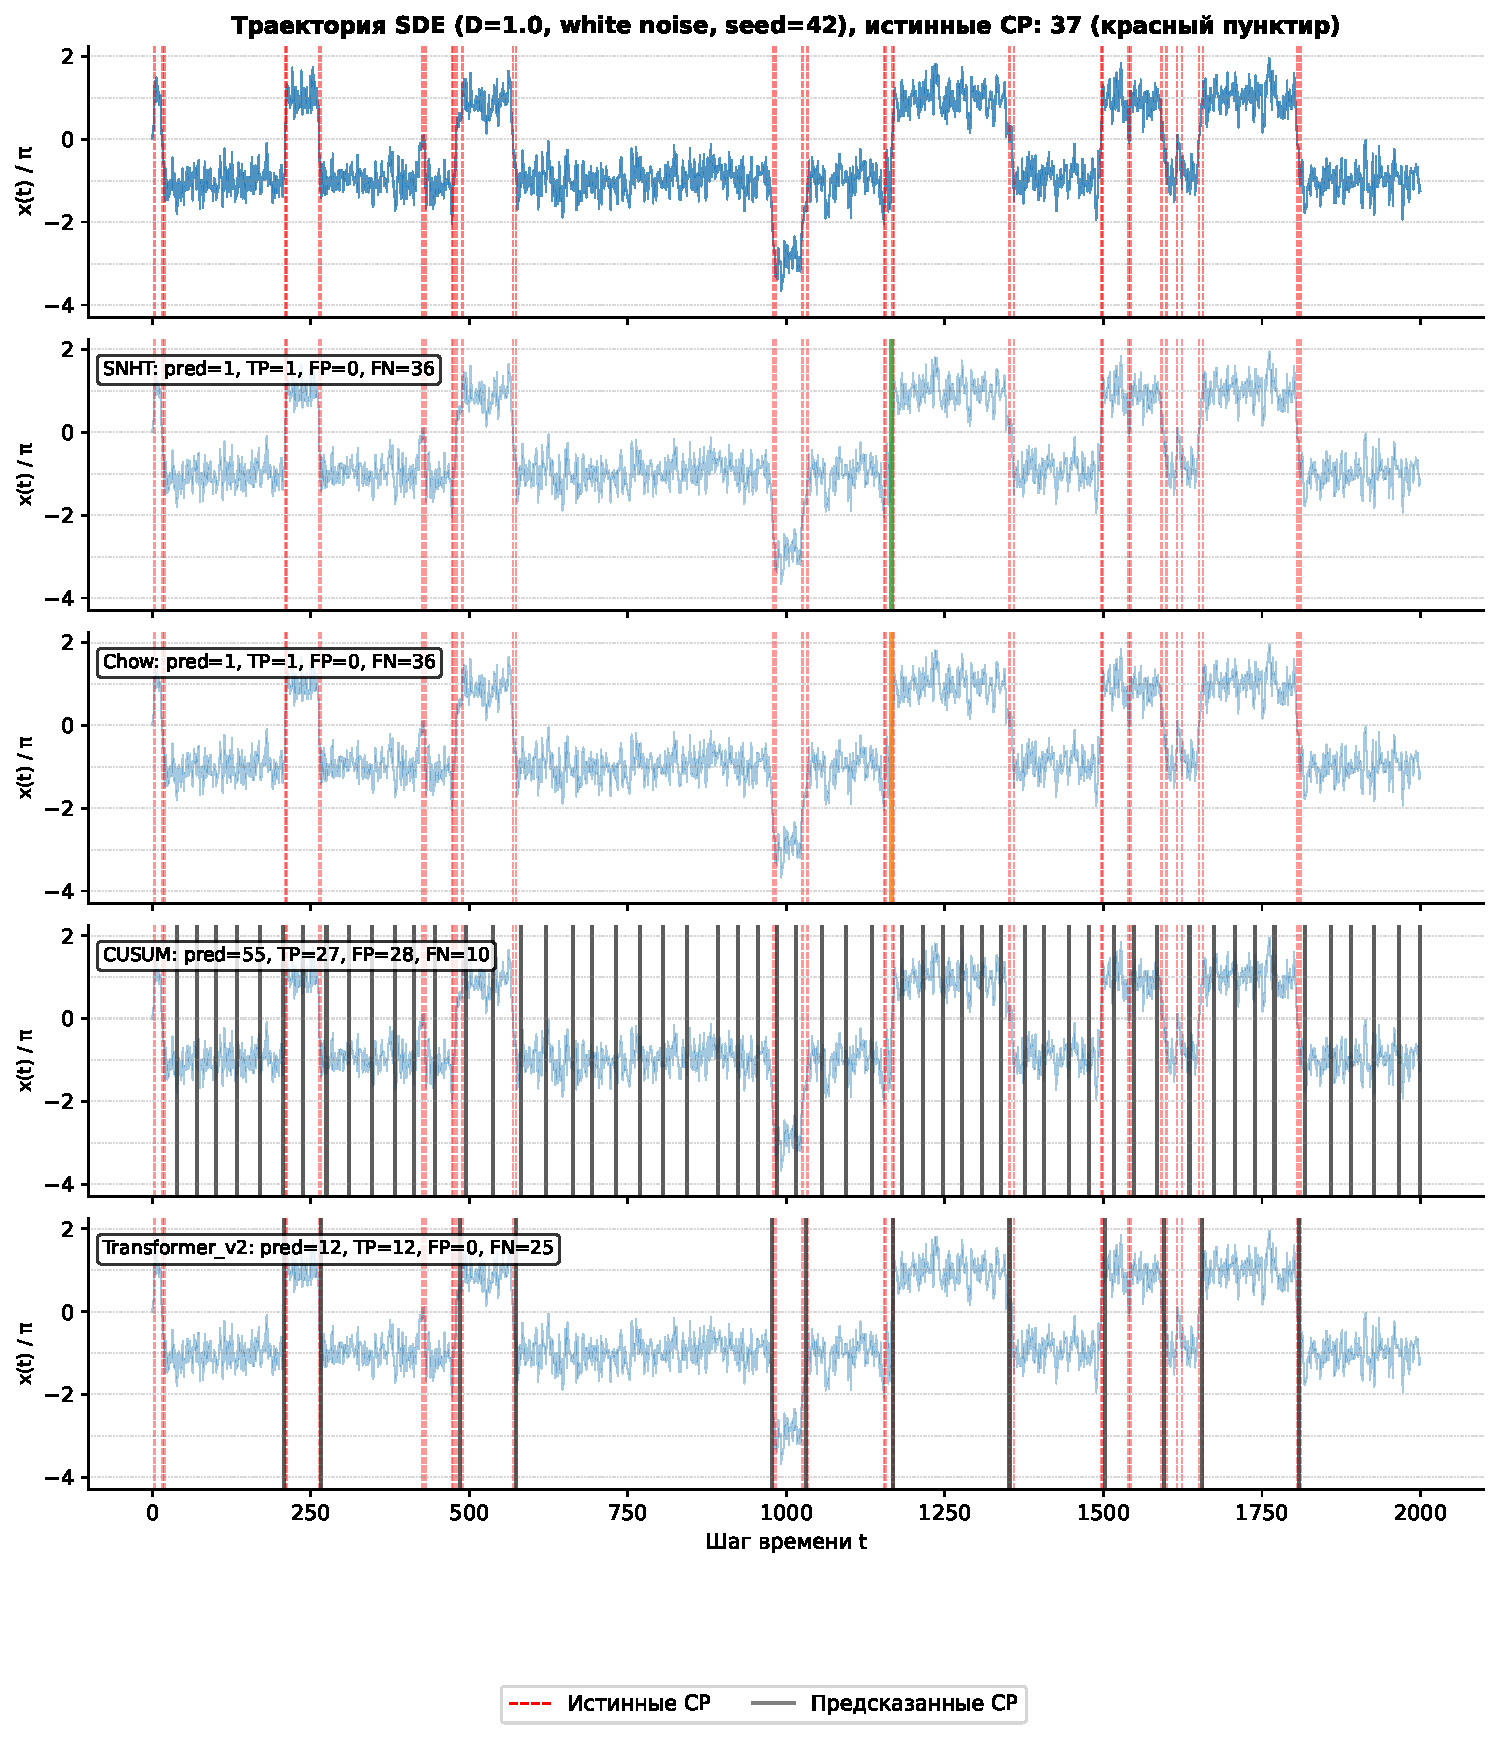
\includegraphics[width=0.95\textwidth]{../figures/example_series.pdf}
\caption{SDE-траектория ($D = 1.0$, белый шум, 2\,000 шагов, 37 истинных CP). Красный пунктир -- истинные точки разладки. Цветные сплошные -- предсказания методов. SNHT и Chow находят по одной точке; CUSUM -- 55 (много ложных); Transformer\_v2 -- 12 (консервативно, но точно).}
\label{fig:example_series}
\end{figure}

\subsection{Метрики качества}

Алгоритм CPD почти никогда не попадает ровно в истинную позицию разладки, поэтому вводится допуск $\delta$: предсказание засчитывается как TP, если расстояние до ближайшей истинной точки не превышает $\delta$ шагов (конкретное значение и процедура сопоставления описаны ниже). На этой основе считаются стандартные метрики:
\begin{equation}
\text{Precision} = \frac{\text{TP}}{\text{TP} + \text{FP}}, \quad
\text{Recall} = \frac{\text{TP}}{\text{TP} + \text{FN}}, \quad
\text{F1} = \frac{2 \cdot \text{Precision} \cdot \text{Recall}}{\text{Precision} + \text{Recall}}
\end{equation}

F1  -- основная метрика; Accuracy не используется (при TN $\gg$ TP алгоритм, всегда отвечающий <<нет>>, получит 99\%+). Для методов с непрерывным score дополнительно считаются \textbf{ROC-AUC} (качество ранжирования без фиксации порога) и \textbf{PR-AUC} (более честная метрика при дисбалансе классов).

Классификационные метрики и метрики локализации мы держим параллельно: на практике точность определения точки и факт детекции  -- разные задачи. Для локализации используется MAE:
\begin{equation}
\text{MAE} = \frac{1}{M}\sum_{i=1}^{M} |\hat{\tau}_i - \tau_i|,
\end{equation}
где $\tau_i$  -- истинное время $i$-й разладки, $\hat{\tau}_i$  -- предсказанное. MAE показывает среднее отклонение в шагах.

\subsection{Разделение данных}

Корректное сравнение методов требует строгого разделения данных на три непересекающихся набора:
\begin{itemize}
    \item \textbf{Обучающий набор} (seeds 0 -- 99): используется только для обучения ML-моделей. Параметры генерации варьируются ($D \in [0.2, 1.0]$, $dt \in \{0.5, 1.0, 2.0\}$, все 5 типов шума), чтобы модели не переобучались на один режим.
    \item \textbf{Калибровочный набор} (seeds 5000 -- 5019, 20 рядов): используется для подбора порогов. Для ML-моделей максимизируется F1 по сетке из 95 значений threshold $\in [0.05, 0.99]$. Для классических тестов используются стандартные уровни значимости.
    \item \textbf{Тестовый набор} (seeds 1000 -- 1049, 50 рядов по 2\,000 шагов): используется только для финального сравнения. Ни один параметр не подбирался на этих данных.
\end{itemize}

Калибровка порогов~ -- критический этап: различия в процедуре калибровки между v1 и v2 описаны в разделе~3.2, влияние на результаты~ -- в разделе~7.

\subsection{Сопоставление и сценарии}

\textbf{Сопоставление предсказаний с истиной.} Предсказанная точка считается верной (TP), если находится в пределах $\delta = 50$ шагов от ближайшей истинной разладки: при $D = 1.0$ среднее расстояние между соседними разладками составляет $\sim$50 шагов, так что $\delta = 50$ означает <<предсказание засчитывается, если оно ближе к правильной разладке, чем к соседней>>. Сопоставление  -- жадное: пары (true, pred) сортируются по расстоянию, каждая точка используется не более одного раза. Непарные предсказания  -- FP, непарные истинные  -- FN. Жадное сопоставление может давать субоптимальные пары по сравнению с венгерским алгоритмом; мы не проверяли разницу формально, но при $\delta = 50$ и типичных расстояниях между CP она пренебрежимо мала.

Допуск $\delta = 50$ не следует путать с NMS-расстоянием (50 для v1-моделей, 10 для v2): $\delta$ используется при сопоставлении предсказаний с разметкой, NMS -- при постобработке score-функции. NMS для v2 уменьшено, поскольку их score-функции менее кластеризованы; $\delta$ при этом не менялся, так как он определяется не свойствами метода, а типичным расстоянием между истинными CP. Единый $\delta = 50$ для всех сценариев  -- осознанный компромисс. При $D = 0.5$ среднее расстояние между CP $\sim$1000 шагов, и $\delta = 50$ составляет лишь 5\% от него  -- допуск очень щедрый. При $D = 1.0$ расстояние $\sim$50 шагов, и $\delta$ совпадает с типичным межпереходным интервалом: предсказание может <<притянуться>> к соседней разладке. Однако жадное сопоставление решает эту проблему  -- ближайшие пары связываются первыми, и каждая точка используется однократно. При $D = 1.5$ расстояние $\sim$17 шагов, и $\delta = 50$ покрывает 2 -- 3 соседних разладки, но опять же однократное использование не позволяет одному предсказанию <<забрать>> несколько истинных точек. Уменьшение $\delta$ ниже 50 наказывало бы методы с неточной локализацией (MAE $> 5$), но не меняло бы ранжирование.

\textbf{Сценарии.} Каждый метод протестирован в четырех условиях: $D = 0.5$ (white), $D = 1.0$ (white), $D = 1.0$ (pink), $D = 1.5$ (white). Это покрывает спектр от тривиальной задачи ($\sim$2 CP на ряд при $D = 0.5$) до сложной ($\sim$115 CP при $D = 1.5$, белый шум; $\sim$191 CP при $D = 1.0$, розовый шум) и позволяет оценить устойчивость методов к типу шума.

\textbf{Статистическая надежность.} 50 независимых реализаций на сценарий дают возможность оценить не только среднее, но и разброс метрик.

\subsection{Устройство пайплайна}

Весь процесс автоматизирован в скрипте \texttt{eval\_multi.py}:
\begin{enumerate}
    \item Генерация тестового ряда с заданными параметрами ($D$, $dt$, noise, seed).
    \item Последовательный запуск всех 18 методов через единый интерфейс.
    \item Сопоставление предсказаний с разметкой, вычисление метрик.
    \item Повторение для 50 сидов, агрегация в \texttt{summary.csv}.
\end{enumerate}

Для ML-моделей адаптер проверяет наличие файла весов и при его наличии пропускает обучение  -- полный eval занимает минуты, а не часы.

\subsection{Исходные гипотезы}

Перед запуском экспериментов сформулированы семь ожиданий, проверяемых в разделе~7:

\begin{enumerate}
    \item Классические тесты лидируют при малом шуме (редкие, выраженные разладки).
    \item ML-модели лидируют при сильном шуме (частые, зашумленные переходы).
    \item Коррелированный шум сильнее бьет по классике, чем по ML.
    \item Существует критический уровень шума, разделяющий режимы.
    \item CUSUM дает высокий recall при низком precision.
    \item Модели v2 значительно лучше v1.
    \item Нейросетевые методы превосходят классику при всех уровнях шума.
\end{enumerate}

\section{Статистический анализ SDE-процесса}

Протокол зафиксирован, но перед запуском детекции мы провели отдельное исследование: как именно устроены переходы в SDE-процессе при разных $D$ и $dt$. Это нужно, чтобы понять, в каком режиме задача тривиальна, а в каком~ -- содержательна, и обосновать выбор тестовых сценариев.

Мы задали себе три вопроса:
\begin{itemize}
    \item Как выглядят <<перелёты>> через границу между впадинами? (H1)
    \item Сколько времени процесс проводит в одной впадине до перескока? (H2)
    \item Случайно ли расположены разладки, или между ними есть зависимость? (H3)
\end{itemize}

\noindent Анализ проведен на сетке из 20 значений~$D$ и 15 значений~$dt$ (всего 300 комбинаций, по 30 рядов на каждую).

\subsection{H1: Перелеты через границу  -- half-normal}

Когда траектория пересекает границу $k\pi$, она <<перелетает>> на некоторое расстояние $|x_t - k\pi|$. Если шум мал, этот перелет определяется одним гауссовским шагом, и его абсолютная величина должна следовать полунормальному распределению (half-normal)  -- это прямое следствие нормальности шумового приращения: $|\xi| \sim \text{half-normal}$ при $\xi \sim \mathcal{N}(0,1)$.

Чтобы проверить, действительно ли перелёты следуют полунормальному распределению, нужен формальный критерий~ -- нельзя просто посмотреть на гистограмму и сказать <<похоже>>. Мы используем критерий согласия хи-квадрат ($\chi^2$). Идея простая: разбиваем наблюдаемые перелёты на интервалы (бины), считаем сколько значений попало в каждый, и сравниваем с тем, сколько \textit{должно было} попасть, если распределение действительно полунормальное. Мера расхождения~ -- статистика $\chi^2 = \sum (O_i - E_i)^2 / E_i$, где $O_i$~ -- наблюдаемое число в $i$-м бине, $E_i$~ -- ожидаемое. Чем больше $\chi^2$, тем хуже совпадение.

По значению $\chi^2$ вычисляется $p$-value~ -- вероятность увидеть такое же или большее расхождение чисто по случайности, если распределение на самом деле полунормальное. Если $p > 0.05$~ -- расхождение легко объяснить случайностью, и у нас нет оснований отвергать гипотезу. Если $p < 0.05$~ -- расхождение слишком велико, полунормальное распределение не подходит.

Формально тест не отвергает гипотезу при малом шуме ($D \leq 0.6$, рис.~\ref{fig:overshoot_heatmap}), но этот результат обманчив: переходов при таком~$D$ мало (десятки -- сотни), и у теста просто недостаточно данных, чтобы отвергнуть что бы то ни было. Гистограмма при $D = 0.2$ (рис.~\ref{fig:overshoot_hist}, левая панель) выглядит рваной и плохо совпадает с теоретической кривой, хотя формально $p = 0.91$.

При более сильном шуме ($D = 1.0$, рис.~\ref{fig:overshoot_hist}, третья панель) ситуация обратная: визуально гистограмма ложится на кривую гораздо лучше, но тест отвергает гипотезу ($p \approx 0$), потому что данных тысячи и даже крошечное отклонение становится <<статистически значимым>>.

Содержательный вывод: полунормальное распределение~ -- разумная аппроксимация перелётов при любом~$D$. Для практики важнее не формальный $p$-value, а сам факт: форма распределения перелётов меняется с~$D$ предсказуемым образом, что помогает выбрать параметры генерации.

\begin{figure}[H]
\centering
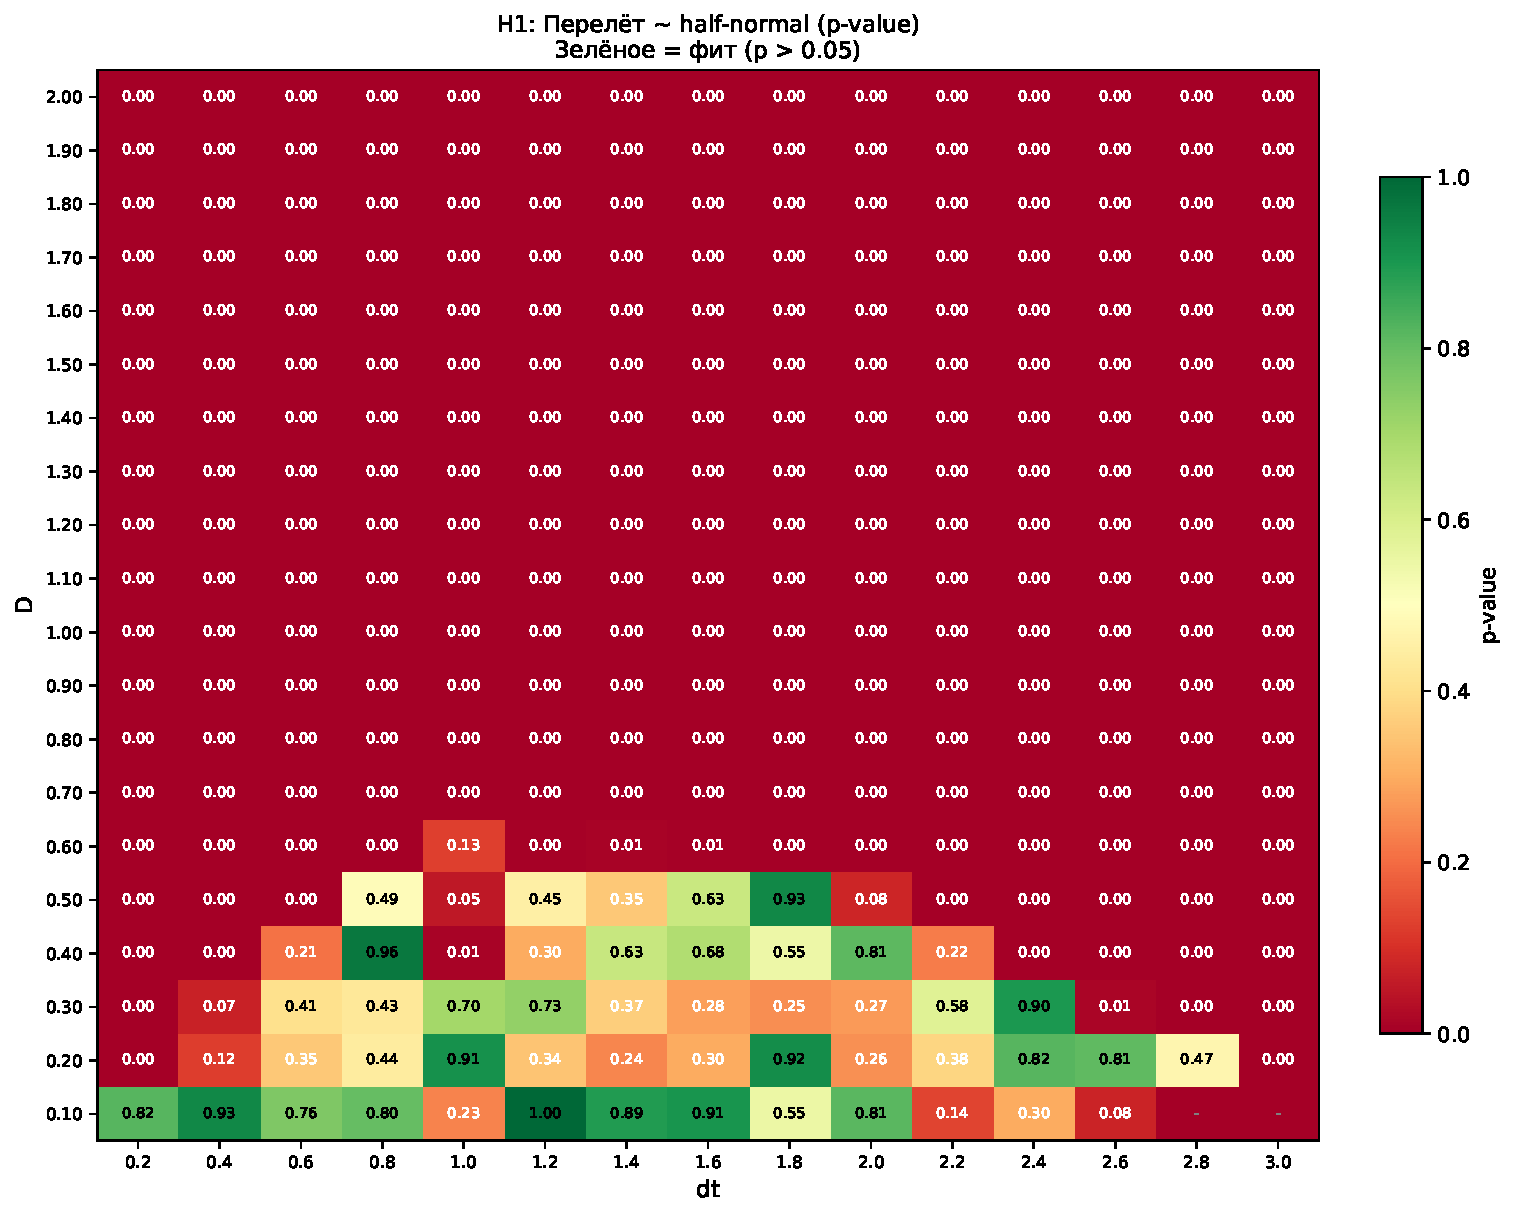
\includegraphics[width=0.7\textwidth]{../figures/overshoot_halfnorm_heatmap.pdf}
\caption{H1: $p$-value хи-квадрат теста на полунормальность перелетов. Зеленые ячейки ($p > 0.05$)  -- гипотеза формально не отвергается, но при малых $D$ это следствие малого объема данных (n = 30 -- 200), а не хорошего совпадения. При $D \geq 1.0$ тест отвергает из-за больших выборок (n $>$ 5000), хотя визуально совпадение лучше (см. рис.~\ref{fig:overshoot_hist}).}
\label{fig:overshoot_heatmap}
\end{figure}

\begin{figure}[H]
\centering
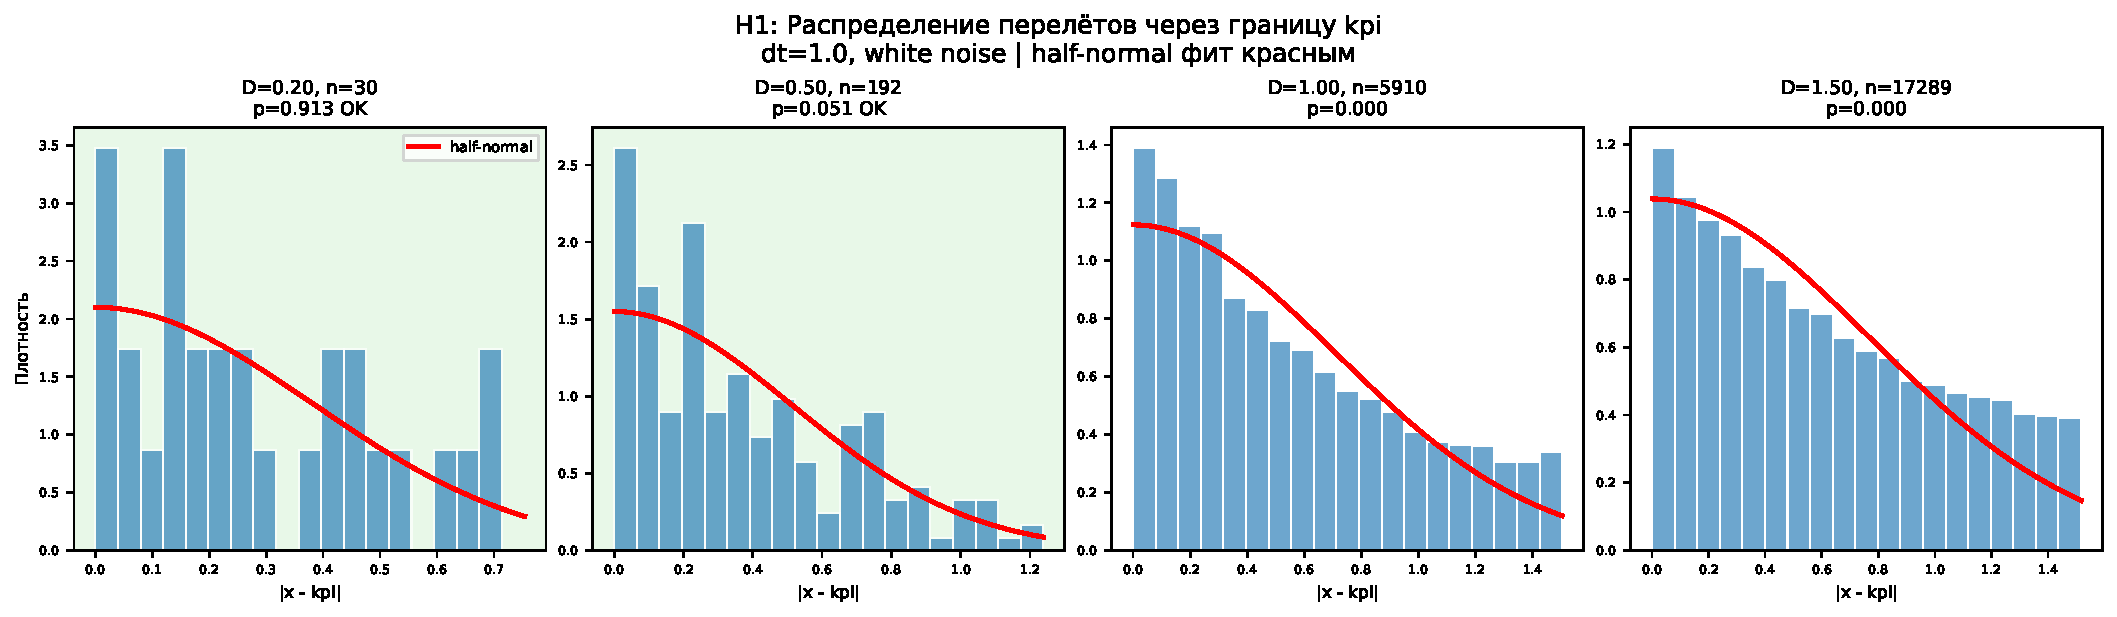
\includegraphics[width=0.95\textwidth]{../figures/overshoot_hist_examples.pdf}
\caption{Гистограммы перелетов через границу $k\pi$ при разных $D$ (dt = 1.0). Красная кривая  -- подгонка полунормальным распределением. При $D = 0.2$ совпадение отличное; при $D = 1.0$ и выше распределение отклоняется.}
\label{fig:overshoot_hist}
\end{figure}

\subsection{H2: Форма распределения временных расстояний между CP}

Сколько времени процесс проводит в одной впадине до перескока в следующую? Чтобы ответить, мы измерили расстояния (в шагах) между последовательными точками разладки и подгоняли к ним гамма-распределение.

Гамма-распределение~ -- гибкое семейство, форма которого управляется одним числом: параметром~$k$ (shape). Этот параметр~ -- удобный индикатор режима процесса:
\begin{itemize}
    \item $k < 1$: распределение скошено вправо~ -- процесс чаще <<перескакивает>> быстро, но иногда застревает надолго.
    \item $k = 1$: экспоненциальное распределение~ -- переходы происходят <<случайно и независимо>>, процесс не <<помнит>>, как давно он в этой впадине.
    \item $k > 1$: колоколообразное~ -- время пребывания сконцентрировано вокруг типичного значения.
\end{itemize}

\noindent На рис.~\ref{fig:transition_hist} видно, как $k$ растёт 
с увеличением шума (значение $k$ указано в заголовке каждой панели):
\begin{itemize}
    \item $D \approx 0.5$, $k \approx 0.27$: распределение сильно скошено вправо -- процесс обычно сидит в одной впадине долго, но изредка перескакивает быстро.
    \item $D \approx 1.0$, $k \approx 0.5$: скошенность уменьшается, гамма-распределение хорошо описывает основное тело данных (рис.~\ref{fig:transition_hist}, вторая панель).
    \item $D \approx 2.0$, $k \approx 1.0$: форма приближается к экспоненциальной -- переходы происходят хаотично, процесс не <<застревает>> надолго.
\end{itemize}

Визуально гамма-распределение описывает данные тем лучше, 
чем больше~$D$: при $D \geq 1.0$ подогнанная кривая практически 
совпадает с гистограммой. При малом~$D$ совпадение хуже~ -- 
данные устроены как смесь двух режимов: короткие осцилляции 
у границы~$\pi$ (процесс перескочил и тут же вернулся) и длинные 
удержания в глубине впадины. Такую смесь одно гамма-распределение 
не описывает, но параметр~$k$ всё равно полезен как индикатор 
режима: его рост от~0.27 до~1.0 отражает переход от редких 
крупных скачков к стационарному потоку мелких переходов.

\begin{figure}[H]
\centering
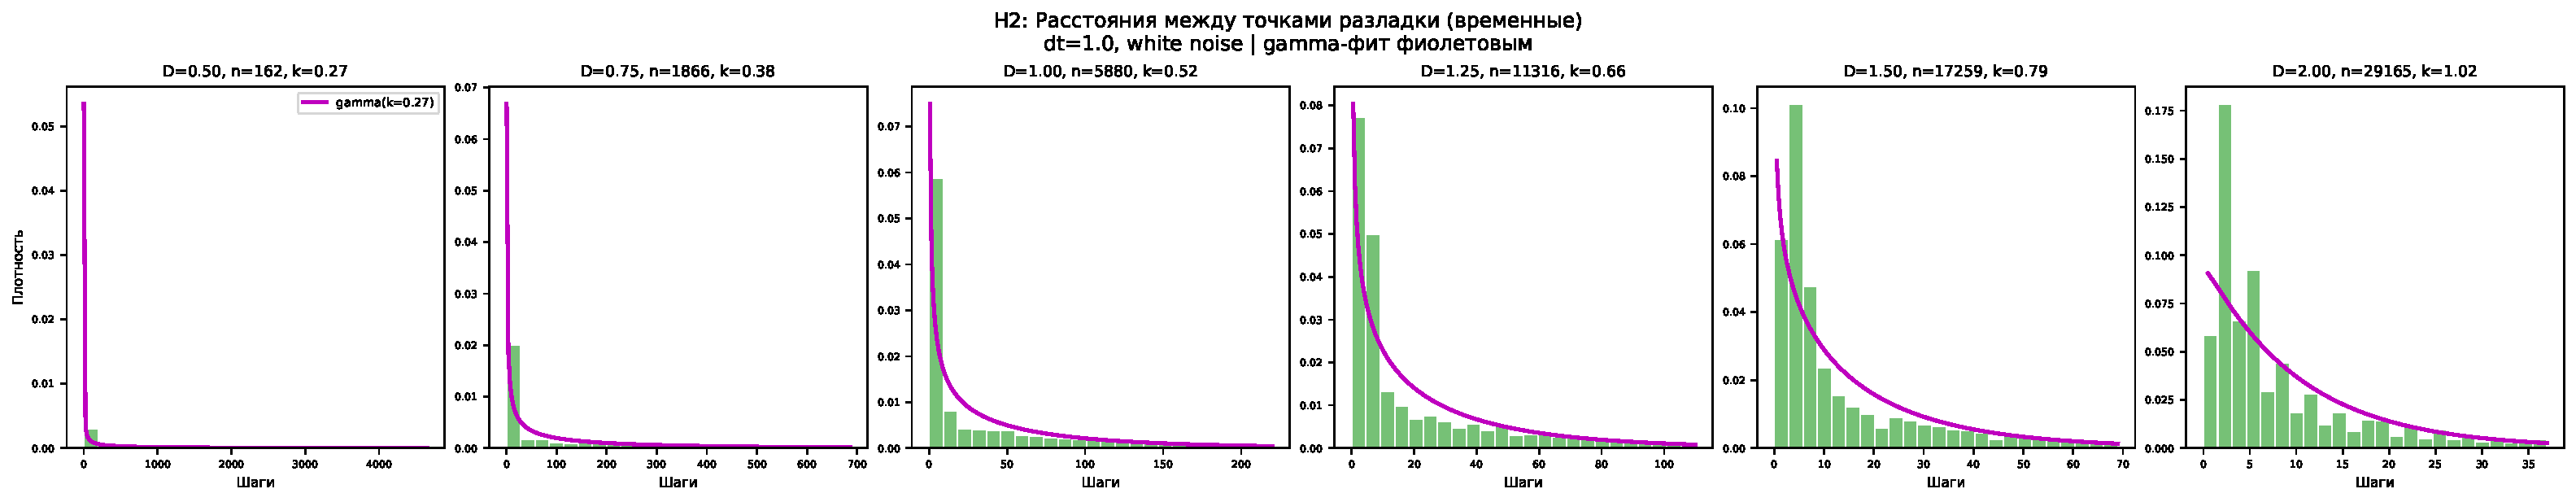
\includegraphics[width=0.95\textwidth]{../figures/transition_hist_examples.pdf}
\caption{Гистограммы временных расстояний между CP при разных $D$. Фиолетовая кривая  -- подгонка гамма-распределением. При малом $D$ распределение сильно скошено вправо, при большом  -- приближается к экспоненциальному.}
\label{fig:transition_hist}
\end{figure}

\subsection{H3: Пуассоновость числа CP}

Случайно ли расположены разладки вдоль ряда, или между ними есть зависимость? Если число переходов на каждом ряде подчиняется распределению Пуассона, это означает, что разладки возникают <<независимо друг от друга>>~ -- как редкие события, не влияющие одно на другое.

Для проверки мы использовали индекс дисперсии~ -- отношение 
дисперсии числа разладок к их среднему числу: 
$DI = \text{Var}(N_{\text{CP}}) / \text{Mean}(N_{\text{CP}})$. 
У пуассоновского распределения дисперсия равна среднему, 
поэтому $DI \approx 1$~ -- признак пуассоновского поведения. 
Отклонения от единицы содержательны: $DI > 1$ 
(передисперсия) означает, что разладки кластеризуются~ -- 
на одних рядах их непропорционально много, на других почти нет; 
$DI < 1$ (недодисперсия)~ -- что разладки распределены 
подозрительно равномерно, как будто между ними есть 
<<отталкивание>>. Для ML-моделей важно именно $DI \approx 1$: 
это гарантирует, что статистики обучающей и тестовой 
выборок будут сопоставимы.

Результат (рис.~\ref{fig:poisson_heatmap}): при достаточном шуме ($D \geq 1.2$) индекс дисперсии стабильно близок к единице ($DI \in [0.8, 1.2]$). Это хорошая новость для ML-моделей: в рабочем диапазоне ($D = 1.0$ -- $1.5$) разладки распределены стационарно, и модель может рассчитывать, что статистики обучения и теста совпадут. При малом~$D$ переходов на ряд слишком мало для осмысленной проверки.

\begin{figure}[H]
\centering
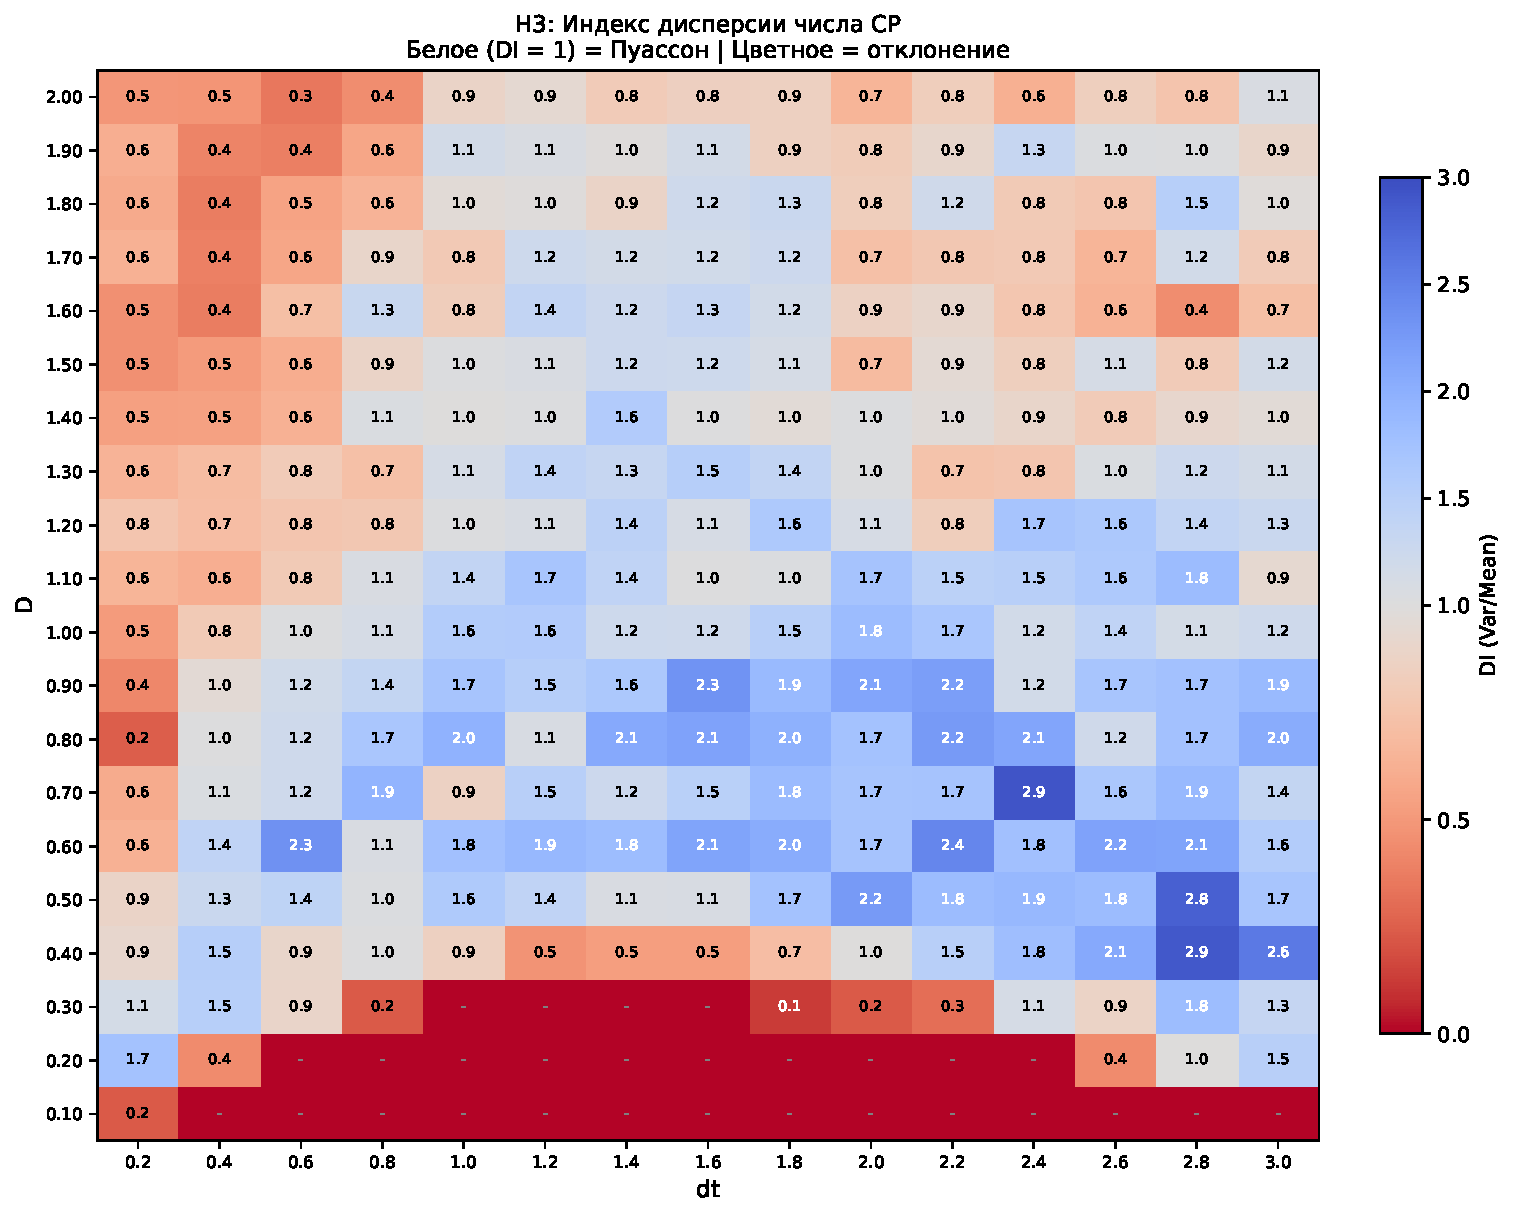
\includegraphics[width=0.7\textwidth]{../figures/poisson_dispersion_heatmap.pdf}
\caption{Индекс дисперсии числа CP: $DI = \text{Var}/\text{Mean}$. Белые ячейки ($DI \approx 1$)  -- пуассоновское поведение. Цветные  -- отклонение: синие ($DI < 1$)  -- недодисперсия или мало данных, красные ($DI > 1$)  -- передисперсия.}
\label{fig:poisson_heatmap}
\end{figure}

\subsection{Сводка гипотез}

Результаты H2 и H3 визуализированы на рис.~\ref{fig:hypothesis_summary}. При малом $D$ переходов мало, распределение расстояний сильно скошено ($k \ll 1$). При большом $D$ поток переходов стационарен ($DI \approx 1$), а распределение приближается к экспоненциальному ($k \to 1$). Зона $D = 1.0$ -- $1.5$ -- промежуточная: переходов достаточно для статистики, но распределение еще далеко от экспоненциального.

\begin{figure}[H]
\centering
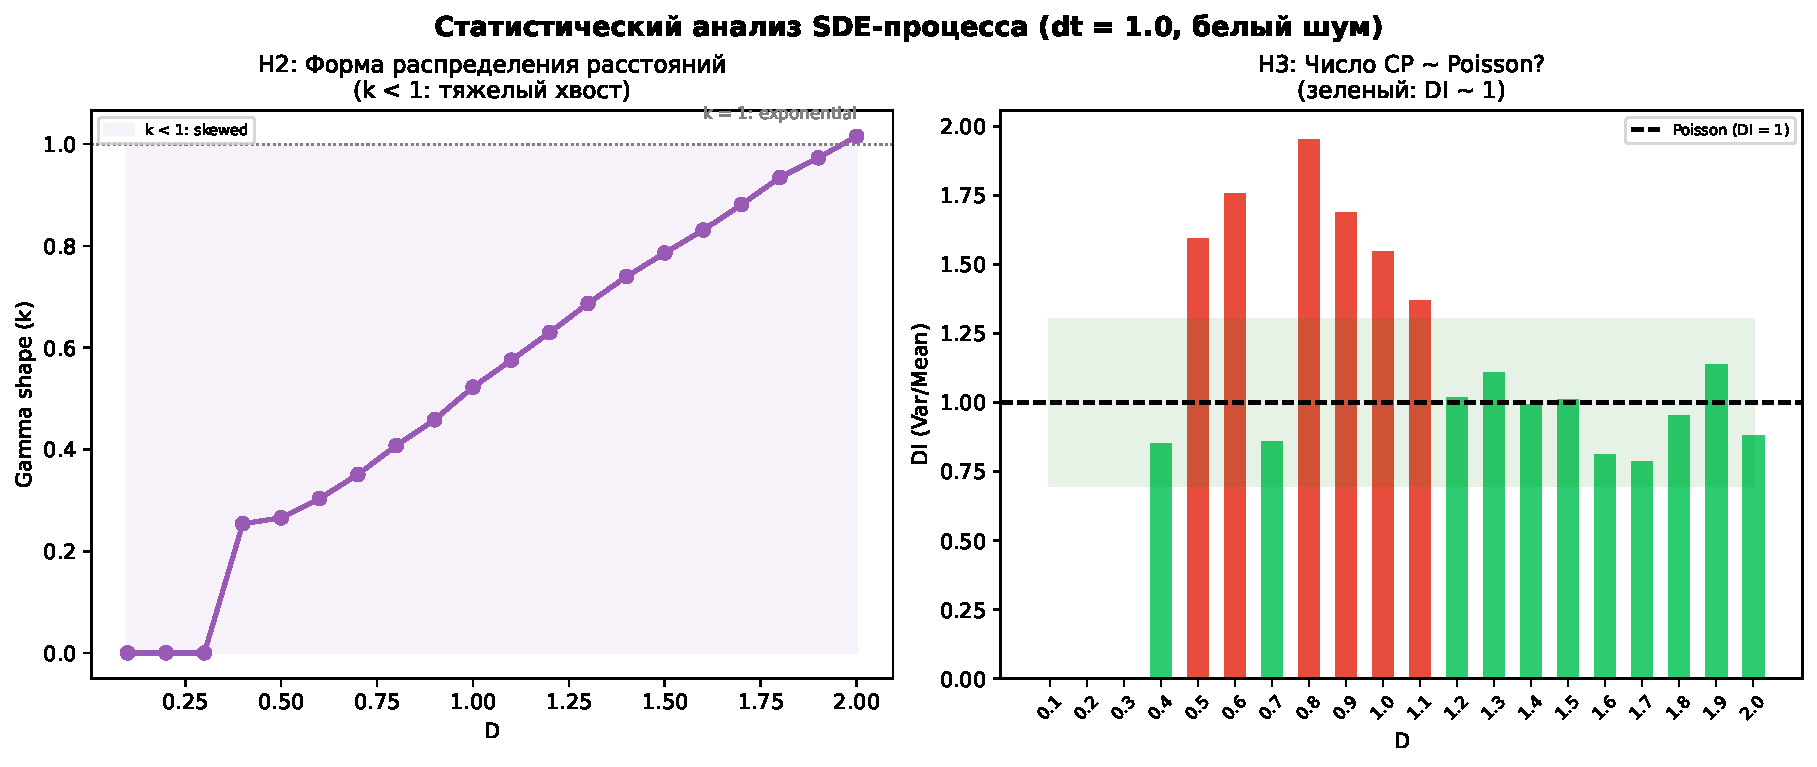
\includegraphics[width=0.95\textwidth]{../figures/hypothesis_summary.pdf}
\caption{Сводка статистического анализа (dt = 1.0, белый шум). Слева: параметр формы $k$ гамма-распределения расстояний между CP (H2). Справа: индекс дисперсии числа CP (H3).}
\label{fig:hypothesis_summary}
\end{figure}

\section{Экспериментальные результаты}

\subsection{Сравнение методов при $D = 1.0$ (рабочий режим)}

Таблица~\ref{tab:d10_white} содержит результаты при $D = 1.0$, белый шум  -- основной режим, в котором задача содержательна.

\begin{table}[ht]
\centering
\caption{Результаты на 50 тестовых рядах, $D = 1.0$, белый шум. Показаны 8 методов с наибольшим F1. Опущены: Buishand (4 варианта, F1 = 0.049), Nyblom (0.049), Pettitt (0.047), GP (0.155), MDL (0.300), SWAB (0.265) и v1-модели (F1 $< 0.40$, см. раздел~3.2). $\sigma$  -- стандартное отклонение F1.}
\label{tab:d10_white}
\begin{tabular}{lcccccc}
\hline
\textbf{Метод} & \textbf{Prec.} & \textbf{Rec.} & \textbf{F1} & $\sigma_{\text{F1}}$ & \textbf{ROC-AUC} & \textbf{PR-AUC} \\
\hline
Transformer\_v2  & 0.77 & \textbf{0.64} & \textbf{0.698} & 0.058 & 0.815 & 0.799 \\
LSTM\_v2         & 0.84 & 0.57 & 0.675 & 0.080 & 0.813 & 0.811 \\
GRU\_v2          & 0.91 & 0.51 & 0.650 & 0.073 & \textbf{0.847} & \textbf{0.850} \\
CUSUM            & 0.46 & \textbf{0.65} & 0.534 & 0.060 & 0.483 & 0.467 \\
CatBoost         & \textbf{0.92} & 0.33 & 0.479 & 0.038 & 0.733 & 0.788 \\
SNHT             & 1.00 & 0.03 & 0.049 & 0.009 &  -- &  -- \\
Chow             & 0.96 & 0.02 & 0.047 & 0.014 & 0.538 & 0.543 \\
Pettitt          & 0.96 & 0.02 & 0.047 & 0.013 &  -- &  -- \\
\hline
\end{tabular}
\end{table}

Три нейросетевых метода v2 уверенно лидируют 
(табл.~\ref{tab:d10_white}). Лучший~ -- Transformer\_v2, 
за ним LSTM\_v2 и GRU\_v2; все три сопоставимы между собой, 
а отрыв от лучшего классического метода (CUSUM) 
устойчив и не объясняется случайным разбросом между рядами. 
Это подтверждает парный тест Уилкоксона~ -- он сравнивает 
F1 каждого метода на одних и тех же 50 рядах и проверяет, 
систематически ли один метод лучше другого: Transformer\_v2 
значимо превосходит CUSUM ($p < 0.0001$), тогда как 
различие между Transformer\_v2 и LSTM\_v2 незначимо 
($p = 0.094$).

Классические тесты SNHT и Chow, которые при $D = 0.5$ были безусловными лидерами (табл.~\ref{tab:d05_white}), здесь практически не работают~ -- recall около 3\%. Причина понятна: при $\sim$200 переходах на ряд однократные тесты на однородность находят лишь один, самый выраженный разрыв. Визуально это хорошо видно на примере SDE-траектории (рис.~\ref{fig:example_series}): SNHT и Chow ставят по одной точке на весь ряд.

CUSUM  -- единственный классический метод, конкурирующий с ML по recall (0.65  -- даже выше, чем у нейросетей), но precision (0.46) хромает  -- слишком много ложных срабатываний. ML-модели, напротив, осторожнее: GRU\_v2 при precision 0.91 пропускает половину переходов, но почти не врет. Компромисс precision -- recall для всех методов показан на рис.~\ref{fig:pr_d10} (справа), а общее ранжирование по F1  -- на рис.~\ref{fig:f1_d10}.

\begin{figure}[H]
\centering
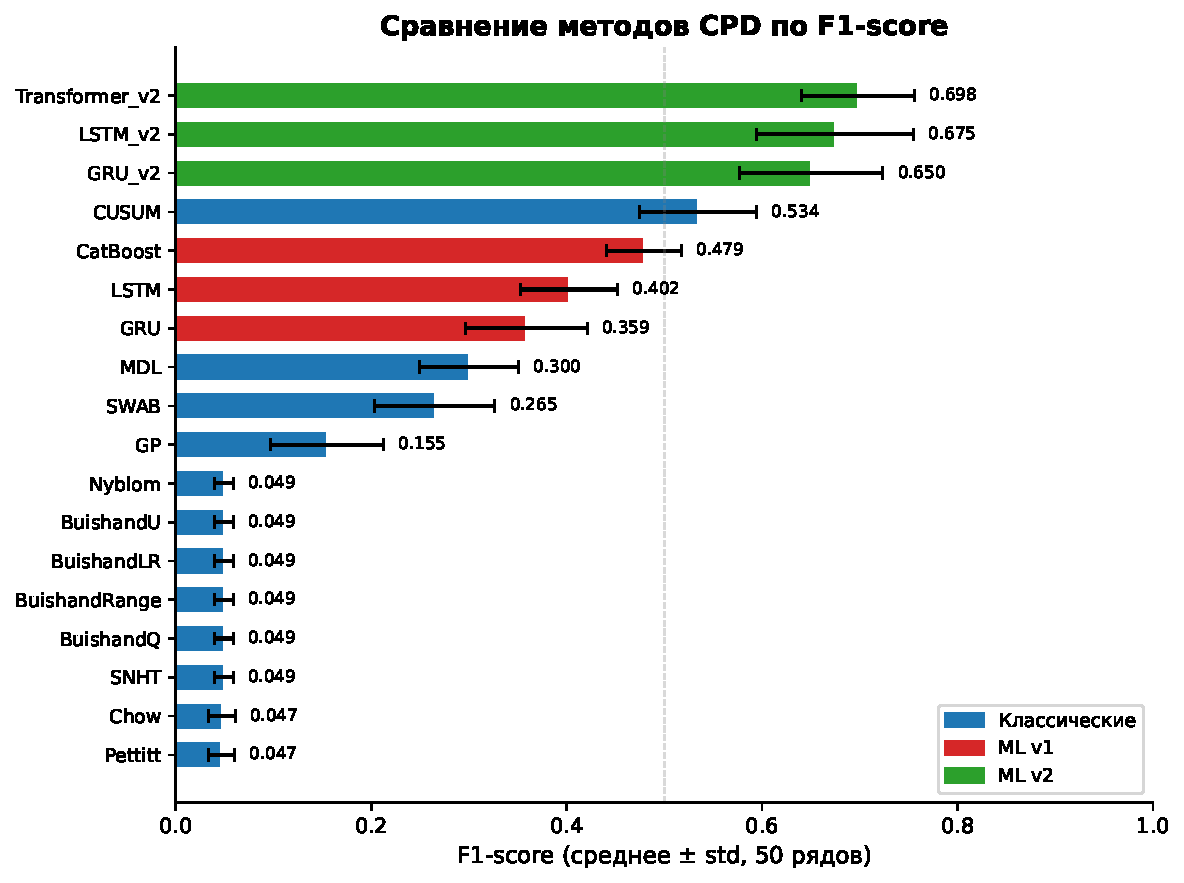
\includegraphics[width=0.85\textwidth]{../figures/f1_comparison_D10.pdf}
\caption{F1-score всех методов при $D = 1.0$, белый шум. ML-модели v2 (зеленые) уверенно лидируют; классические тесты (синие) показывают recall $< 3\%$.}
\label{fig:f1_d10}
\end{figure}

\subsection{Сравнение при $D = 0.5$ (простой режим)}

Результаты при $D = 0.5$ приведены в табл.~\ref{tab:d05_white}.

\begin{table}[ht]
\centering
\caption{Результаты на 50 тестовых рядах, $D = 0.5$, белый шум.}
\label{tab:d05_white}
\begin{tabular}{lccccc}
\hline
\textbf{Метод} & \textbf{Precision} & \textbf{Recall} & \textbf{F1} & \textbf{ROC-AUC} & \textbf{PR-AUC} \\
\hline
SNHT             & \textbf{1.00} & \textbf{0.64} & \textbf{0.725} &  -- &  -- \\
Chow             & 0.92 & 0.56 & 0.645 & 0.684 & 0.533 \\
GRU\_v2          & 0.32 & 0.23 & 0.253 & \textbf{0.919} & \textbf{0.551} \\
CatBoost         & 0.36 & 0.21 & 0.243 & 0.650 & 0.211 \\
LSTM\_v2         & 0.24 & 0.21 & 0.207 & 0.866 & 0.424 \\
Buishand (LR)    & 0.44 & 0.13 & 0.205 & 0.486 & 0.173 \\
\hline
\end{tabular}
\end{table}

SNHT (F1 = 0.725) и Chow (F1 = 0.645) превосходят ML-модели с большим отрывом (рис.~\ref{fig:pr_d10}, слева). Recall SNHT = 0.64 может показаться неожиданным для теста, который ищет ровно одну точку: при $\sim$2 CP на ряд recall усредняется по рядам, и на рядах с 1 CP SNHT получает recall = 1.0, а на рядах с 3+ CP -- recall падает до 0.33 и ниже. В среднем по 50 рядам это дает 0.64. При $\sim$11 переходах на 10\,000 шагов задача сводится к поиску единичного сдвига в почти стационарном ряде -- именно то, для чего создавались тесты на однородность. ML-модели, обученные на рядах с десятками и сотнями переходов, здесь не в своей стихии.

ROC-AUC у GRU\_v2 (0.919) и LSTM\_v2 (0.866) при $D = 0.5$ остается высоким -- модели <<чувствуют>> разладки, но их пороги, откалиброванные на более шумных данных, слишком агрессивны. При подборе порога отдельно под $D = 0.5$ F1 был бы существенно выше, но это требует знания $D$ заранее, чего на практике обычно нет.

\subsection{Влияние типа шума и уровня диффузии}

Рис.~\ref{fig:f1_scenarios} показывает F1-score ключевых методов по четырем сценариям. Видно, что Transformer\_v2 стабильно лидирует при $D \geq 1.0$, а при розовом шуме ($D = 1.0$, pink) его преимущество даже усиливается: коррелированный шум затрудняет работу классических тестов, но не мешает нейросетям.

\begin{figure}[H]
\centering
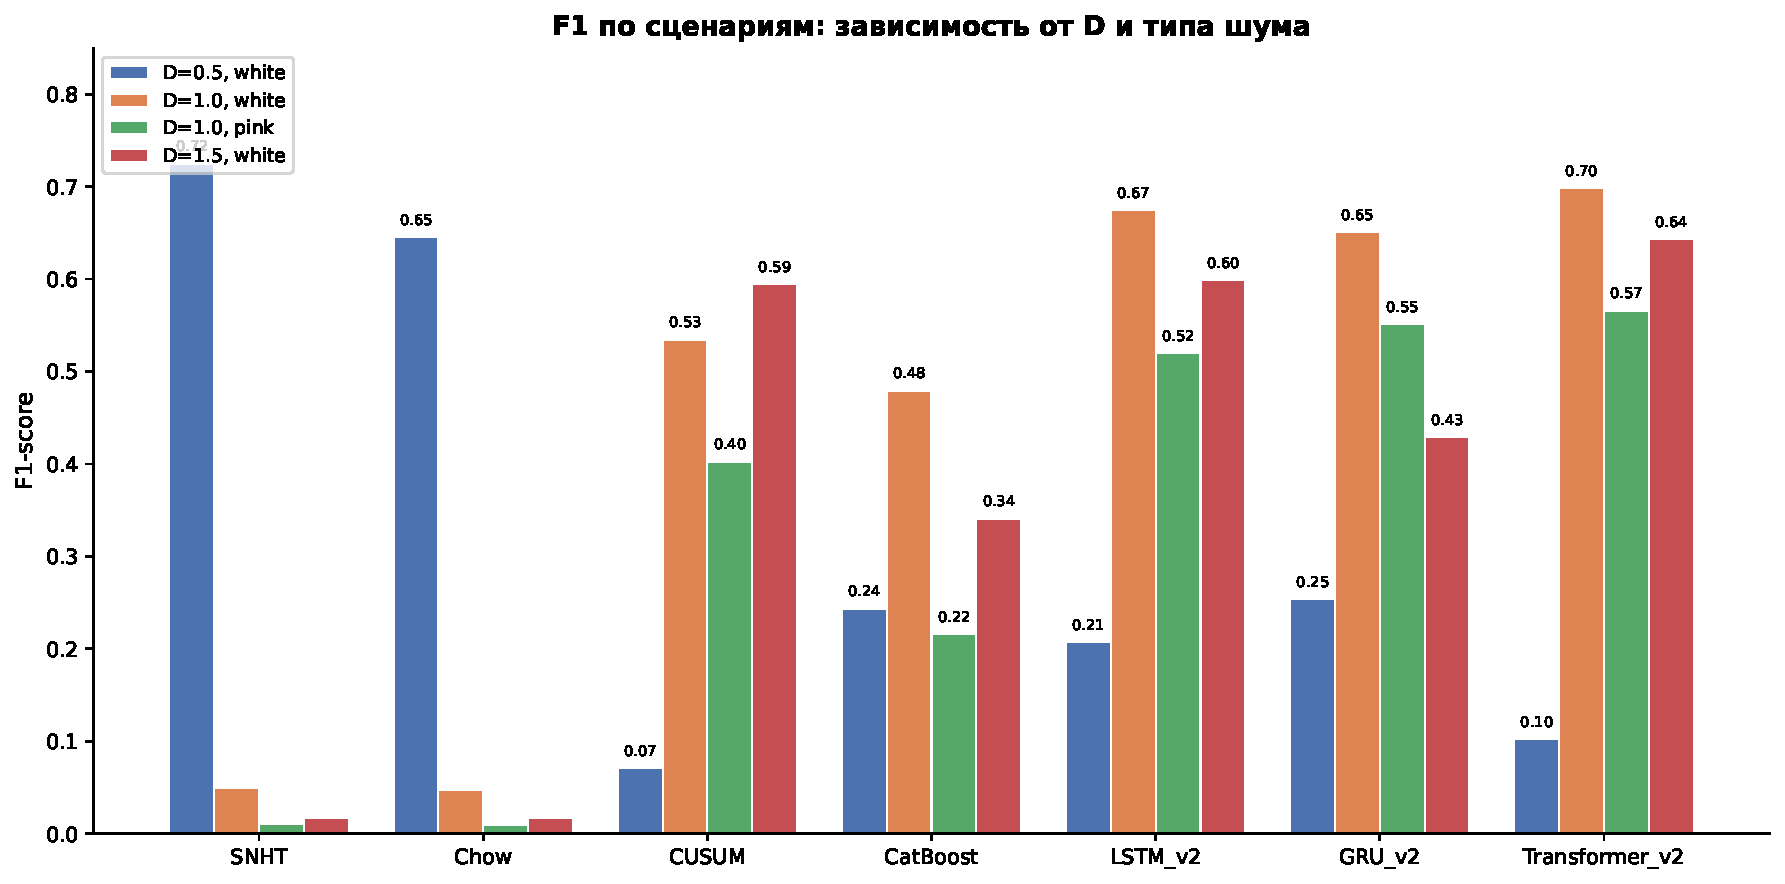
\includegraphics[width=0.85\textwidth]{../figures/f1_scenarios.pdf}
\caption{F1-score ключевых методов по четырем сценариям: $D = 0.5$ (white), $D = 1.0$ (white и pink), $D = 1.5$ (white).}
\label{fig:f1_scenarios}
\end{figure}

Другой ракурс  -- ROC-AUC, который оценивает качество score-функции без привязки к конкретному порогу. На рис.~\ref{fig:roc_scenarios} видно, что ML-модели v2 стабильно держат ROC-AUC выше 0.80 во всех сценариях, тогда как CUSUM и CatBoost заметно просаживаются. Это говорит о том, что сами score-функции нейросетей информативны  -- вопрос лишь в правильном выборе порога.

\begin{figure}[H]
\centering
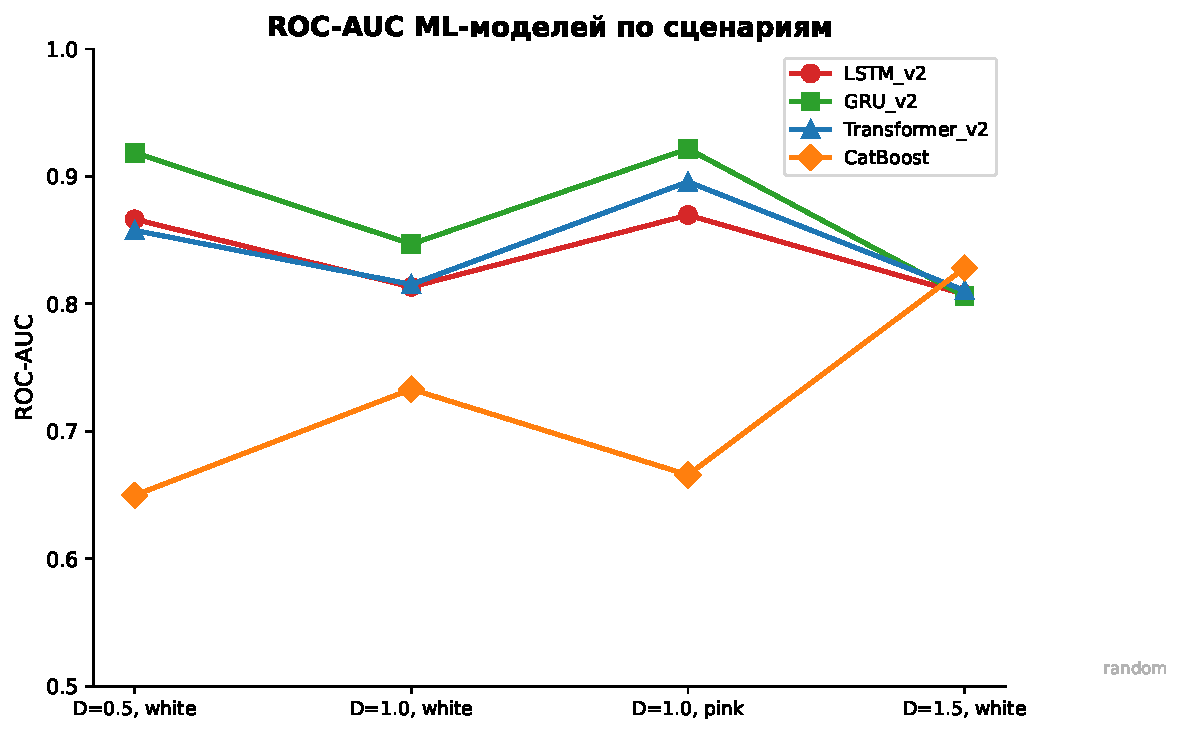
\includegraphics[width=0.85\textwidth]{../figures/roc_auc_scenarios.pdf}
\caption{ROC-AUC ML-методов по четырем сценариям. Модели v2 сохраняют высокое качество ранжирования даже при смене параметров генерации.}
\label{fig:roc_scenarios}
\end{figure}

Компромисс precision -- recall показан на рис.~\ref{fig:pr_d10}: каждый метод занимает свою нишу  -- от <<осторожных>> (высокий precision, низкий recall) до <<агрессивных>> (наоборот).

\begin{figure}[H]
\centering
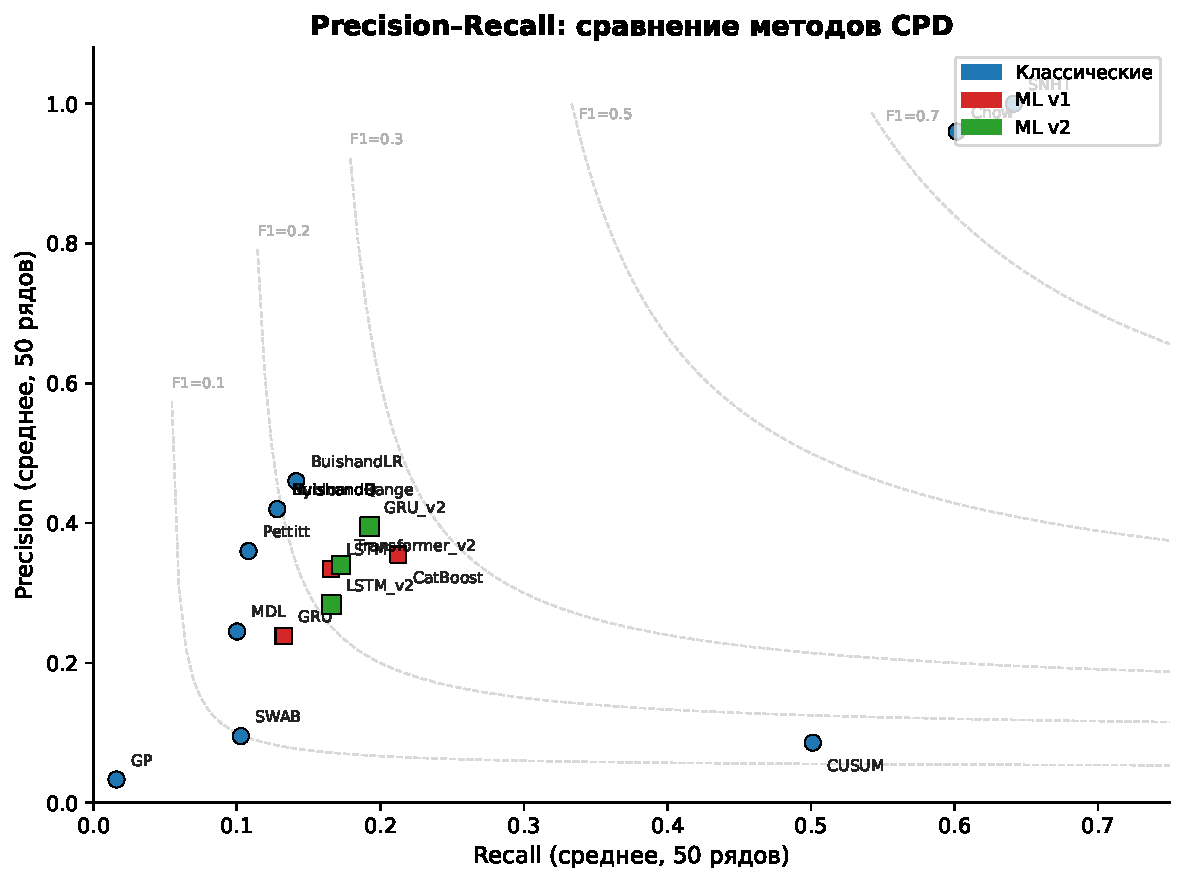
\includegraphics[width=0.48\textwidth]{../figures/precision_recall_D05.pdf}
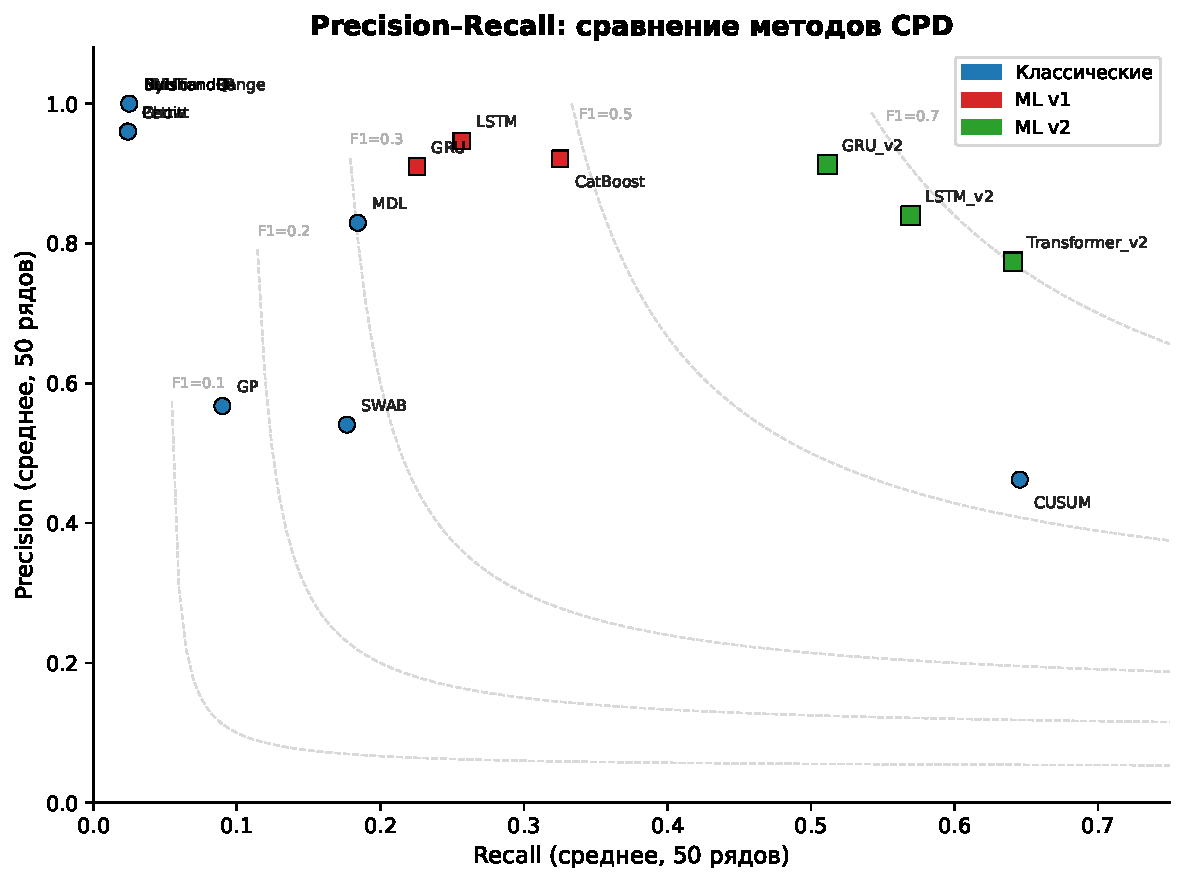
\includegraphics[width=0.48\textwidth]{../figures/precision_recall_D10.pdf}
\caption{Scatter-диаграмма Precision -- Recall для $D = 0.5$ (слева) и $D = 1.0$ (справа). Изолинии  -- уровни F1.}
\label{fig:pr_d10}
\end{figure}

\subsection{Точность локализации}

Для методов, которые детектируют разладки, важно не только <<нашел/не нашел>>, но и <<насколько точно>>. Средняя абсолютная ошибка локализации (MAE) показывает, на сколько шагов предсказание отстоит от истинной позиции разладки (рис.~\ref{fig:mae}).

При $D = 1.0$ лучшую точность локализации показали GRU (MAE = 1.5 шага) и CatBoost (MAE = 2.3 шага) -- при условии, что детекция состоялась. LSTM\_v2 и Transformer\_v2 дали MAE около 3.4 -- 3.6. Когда ML-методы находят разладку, они попадают с точностью до нескольких шагов -- значительно лучше, чем CUSUM (MAE = 9.8), который <<видит>> разладки, но локализует их неточно.

\begin{figure}[H]
\centering
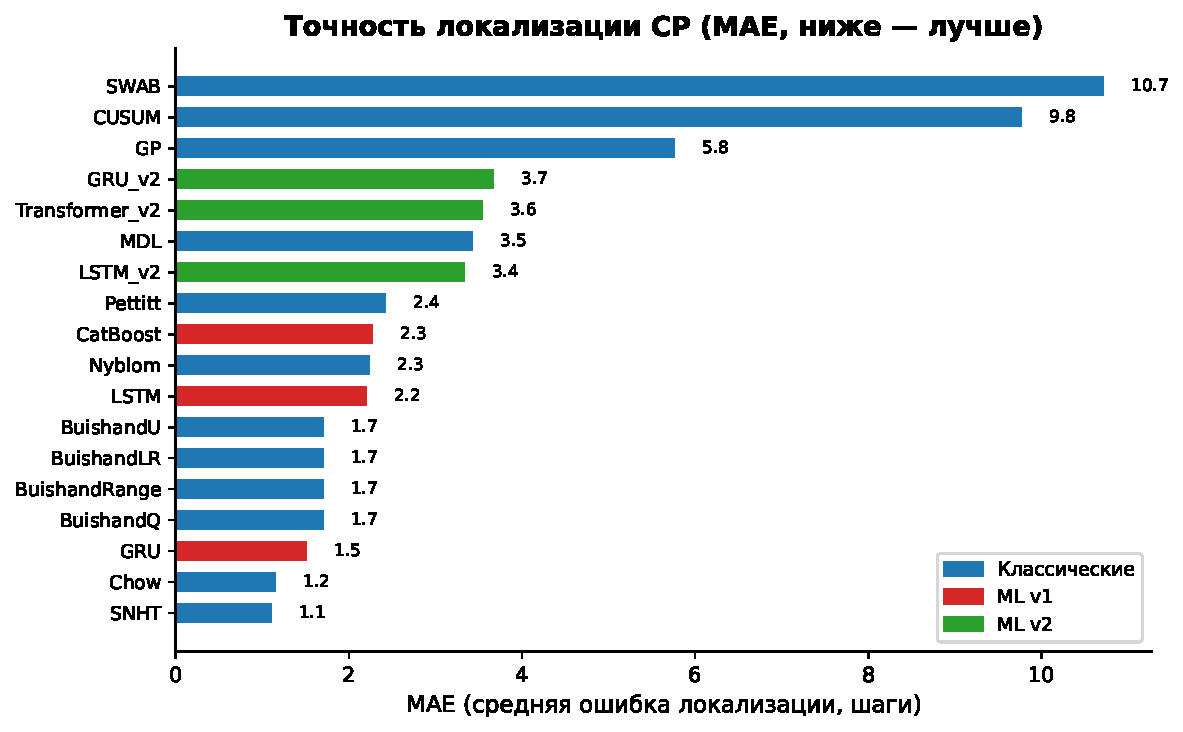
\includegraphics[width=0.7\textwidth]{../figures/mae_comparison.pdf}
\caption{Средняя абсолютная ошибка локализации (MAE) для методов с MAE $< 50$.}
\label{fig:mae}
\end{figure}

\subsection{Сводка по сценариям}

Таблица~\ref{tab:summary_scenarios} собирает лучшие результаты по классам методов через все четыре сценария.

\begin{table}[ht]
\centering
\caption{Лучший классический и лучший ML-метод по F1 в каждом сценарии (50 тестовых рядов по 2\,000 шагов).}
\label{tab:summary_scenarios}
\begin{tabular}{lcccc}
\hline
\textbf{Сценарий} & \textbf{Лучший классич.} & \textbf{F1} & \textbf{Лучший ML} & \textbf{F1} \\
\hline
$D = 0.5$, white & SNHT & \textbf{0.725} & GRU\_v2 & 0.253 \\
$D = 1.0$, white & CUSUM & 0.534 & Transformer\_v2 & \textbf{0.698} \\
$D = 1.0$, pink  & CUSUM & 0.402 & Transformer\_v2 & \textbf{0.566} \\
$D = 1.5$, white & CUSUM & 0.595 & Transformer\_v2 & \textbf{0.643} \\
\hline
\end{tabular}
\end{table}

При $D = 0.5$ классика выигрывает с большим отрывом. При $D \geq 1.0$ ML-методы стабильно лидируют (рис.~\ref{fig:f1_scenarios}). CUSUM  -- единственный классический метод, конкурентоспособный в сложных сценариях, но уступающий Transformer\_v2 на 0.05 -- 0.16 по F1.

\section{Интерпретация и обсуждение}

\subsection{Почему разные методы побеждают в разных режимах}

При $D \geq 1.0$ задача -- распознавание сложных паттернов: осцилляции у границы $\pi$, последовательности быстрых переходов, наложение дрифта и шума. Нейросети обучаются на примерах таких паттернов. Transformer\_v2 оказался лучшим (F1 = 0.698), LSTM\_v2 сопоставим (0.675), GRU\_v2 чуть хуже (0.650). Разница между Transformer\_v2 и LSTM\_v2 статистически пограничная, а вот между тройкой v2 и остальными методами -- значимая.

При $D = 0.5$ картина обратная: переходов мало, они ярко выражены, и SNHT с Chow оптимально заточены именно под это -- один четкий сдвиг в стационарном ряде. ML-модели, обученные на данных с десятками переходов, <<галлюцинируют>> -- находят лишние разладки, снижая precision. Причина не в теоретических ограничениях нейросетей, а в несоответствии обучающего и тестового режимов.

\subsection{Режимный анализ}

Сформулируем практические рекомендации (задача~5). 
Статистический анализ SDE-процесса (раздел~6, 
рис.~\ref{fig:hypothesis_summary}) позволяет связать 
свойства данных с оптимальным методом. Ключевые индикаторы~ -- 
параметр формы~$k$ гамма-распределения межпереходных 
расстояний и индекс дисперсии~$DI$ числа разладок:
\begin{itemize}
    \item \textbf{Малый шум} ($D < 0.7$, $k < 0.4$): 
    переходов мало, они хорошо выражены~ -- применять 
    классические тесты (SNHT, Chow). ML-модели здесь 
    проигрывают не потому, что не <<чувствуют>> разладки 
    (ROC-AUC у GRU\_v2 при $D = 0.5$ составляет 0.919), 
    а потому, что их пороги откалиброваны на более шумные 
    данные. При повторном подборе порога под конкретный~$D$ результат 
    будет лучше, но в этом режиме классика и так справляется.
    \item \textbf{Рабочий режим} ($D \in [1.0, 1.5]$,
    $k \approx 0.5$ -- $0.8$; $DI \approx 1$ при $D \geq 1.2$): разладки 
    образуют стационарный поток, задача нетривиальна~ -- 
    применять ML (Transformer\_v2 или LSTM\_v2).
    \item \textbf{Сильный шум} ($D > 1.8$, $k \to 1$): 
    время пребывания во впадине становится экспоненциальным, 
    переходы независимы. Задача формально проще, но 
    разладки идут так плотно, что практическая полезность 
    детекции снижается.
\end{itemize}

\noindent Граница между <<территорией классики>> и 
<<территорией ML>> лежит в районе $D \approx 0.7$ -- $1.0$. 
Статистический порог ($D \leq 0.6$ из анализа перелётов, 
раздел~6.1) и экспериментальный ($D < 0.7$ из сравнения 
методов) не совпадают точно; зона $D \in [0.6, 0.7]$~ -- 
переходная.

\subsection{Анализ ошибок}

Средние метрики скрывают структуру ошибок. Чтобы понять, \textit{как именно} ошибаются разные методы, посмотрим на типичный ряд при $D = 1.0$ (белый шум, в среднем $\sim$40 истинных разладок):
\begin{itemize}
    \item \textbf{Transformer\_v2} предсказывает 34 точки, из которых $\sim$8 ложных и $\sim$15 пропущенных~ -- сбалансированный профиль ошибок.
    \item \textbf{CUSUM} выдаёт 57 предсказаний: находит больше всех (recall 0.65), но 31 из них ложные~ -- <<шумный>> детектор.
    \item \textbf{GRU\_v2} осторожнее всех: 23 предсказания, из них ложных всего 2, зато пропущено 20~ -- <<тихий>> детектор.
\end{itemize}

Здесь стоит оговориться: F1 неявно предполагает равную цену 
ложной тревоги и пропуска. На практике это не всегда так. 
Однако у ML-моделей есть преимущество: непрерывный score 
позволяет сдвигать порог~$\theta$ и перемещаться вдоль всей 
кривой precision -- recall. Если пропустить разладку дорого~ -- 
достаточно снизить порог, и recall вырастет за счёт precision. 
Высокий ROC-AUC у Transformer\_v2 (0.815) гарантирует, что 
при любом выбранном компромиссе он будет лучше CUSUM, у 
которого ROC-AUC всего 0.483. Классические single-CP тесты 
(SNHT, Chow) такой гибкости лишены~ -- они выдают одну точку 
и не имеют настраиваемого порога.

В худших случаях Transformer\_v2 проседает до F1 $\approx$ 0.56 -- 0.60. Это происходит на рядах, где процесс активно осциллирует вблизи границы $\pi$, не совершая <<настоящего>> перехода  -- модель принимает эти колебания за разладки. CUSUM страдает от той же проблемы, но сильнее, потому что реагирует на любой сдвиг среднего, а SDE-процесс вблизи $\pi$ дает ложные сдвиги постоянно.

\subsection{Вычислительная сложность}

На наших рядах (2\,000 шагов, Kaggle T4 GPU) инференс всех методов укладывается в секунды: классические тесты  -- доли секунды (кроме SNHT: $\sim$4 с (полный перебор позиций разделения)), CatBoost и GRU  -- доли секунды, Transformer\_v2  -- около 0.8 секунды. Обучение  -- другой вопрос: CatBoost обучается за 1 -- 2 минуты на CPU, рекуррентные сети  -- за 10 -- 30 минут на GPU, Transformer\_v2  -- около часа. Если веса уже есть, все ML-методы работают так же быстро, как классика. Таким образом, выбор между классикой и ML определяется не вычислительными затратами, а свойствами данных (см. раздел~8.3).

\subsection{Ограничения}

Работа проведена на синтетических данных одного типа (SDE с $\sin$-потенциалом). Это сознательный выбор, дающий полный контроль над параметрами, но ограничивающий генерализацию: мы не знаем, как методы поведут себя на SDE с другим потенциалом (например, $V(x) = x^4 - x^2$) или на многомерных процессах. Реальные ряды устроены иначе, и перенос выводов требует проверки.

Для контекста: на стандартных кусочно-стационарных бенчмарках нейросетевые методы CPD достигают F1 порядка 0.80 -- 0.90 \cite{truong2020, hushchyn2020}. На наших SDE-данных потолок ниже -- 0.698 при $D = 1.0$. Это отражает повышенную сложность задачи: разладки здесь не скачки между двумя уровнями, а переходы через потенциальный барьер, маскируемые шумом.

Отдельно стоит отметить низкий F1 у Transformer\_v2 при 
$D = 0.5$ (0.102~ -- худший среди ML). Это не ограничение 
архитектуры, а следствие обучающей выборки: модель 
тренировалась на рядах с десятками переходов и при 
$D = 0.5$ <<галлюцинирует>> лишние (precision 0.06). 
GRU\_v2 в том же режиме показывает ROC-AUC = 0.919~ -- 
нейросети \textit{способны} детектировать разладки при 
малом шуме, но для этого нужна повторный подбор порога 
или переобучение на соответствующем~$D$. Если~$D$ 
известен заранее, специализированная ML-модель, 
вероятно, догонит классику; если нет~ -- SNHT надёжнее.

\section{Заключение}

Мы получили два конкретных правила. Первое: при $D < 0.7$ 
нейросети в универсальной конфигурации (обученные на широком 
диапазоне~$D$) уступают простому SNHT; для конкуренции 
с классикой им нужен повторный подбор порога или переобучение под 
конкретный режим. Второе: при $D \geq 1.0$ Transformer\_v2 
выигрывает у лучшего классического метода (CUSUM) на 0.16 
по F1, и это подтверждается парным тестом Уилкоксона 
($p < 0.0001$). Граница между этими режимами~ -- район 
$D \approx 0.7$ -- $1.0$~ -- определена экспериментально 
и подтверждена статистическим анализом SDE-процесса.

Три наблюдения, которые мы не ожидали. Во-первых, самый 
большой прирост качества ML-моделей дала не архитектура 
и не объём данных, а приведение в соответствие статистик 
обучающей и тестовой выборок (v1~$\to$~v2, рост F1 
на 0.3 -- 0.5). Во-вторых, CUSUM~ -- метод 1954 года~ -- 
при $D = 1.0$ показал recall выше, чем любая нейросеть. 
Он проиграл по F1 только из-за precision, а не из-за 
чувствительности. В-третьих, ML-модели <<чувствуют>> 
разладки даже в режиме, где проигрывают по F1: ROC-AUC 
у GRU\_v2 при $D = 0.5$ составляет 0.919, что означает 
существование порога, при котором модель работает 
хорошо~ -- просто текущий порог не тот. Это важно 
практически: имея непрерывный score, ML-модель можно 
настроить на любой компромисс precision -- recall, тогда 
как классические single-CP тесты такой гибкости лишены.

На SDE-данных лучший достигнутый F1 составляет 0.698
(против 0.80 -- 0.90 на стандартных бенчмарках). Разрыв 
отражает повышенную сложность задачи: разладки здесь 
не скачки между двумя уровнями, а переходы через 
потенциальный барьер, маскируемые шумом. Статистический 
анализ процесса (параметр формы~$k$ межпереходных 
расстояний, индекс дисперсии числа CP) показал, при каких 
параметрах задача тривиальна, а при каких содержательна. 
Это может быть полезно при проектировании SDE-генераторов 
для задач CPD.

\textbf{Воспроизводимость.} Все эксперименты воспроизводимы: 
фиксированные seeds для генерации (train 0 -- 99, val 5000 -- 5019, 
test 1000 -- 1049), единый конфиг (\texttt{configs/base.yaml}), 
предобученные веса в репозитории. Полный eval запускается 
одной командой (\texttt{python eval\_multi.py -- n-series 50}) 
и занимает несколько минут при наличии весов.

\textbf{Ход работы.} Проект шёл не линейно. Первые эксперименты проводились при $D = 0.5$, где классические тесты уверенно лидируют, и ранний вывод был: нейросети не нужны. Лишь после перехода к $D = 1.0$ картина изменилась на противоположную. Аналогично, наибольший прирост качества ML-моделей дала не смена архитектуры (разница между LSTM, GRU и Transformer составила 0.02--0.05 по F1), а исправление состава обучающей выборки (v1~$\to$~v2, рост F1 в 1.7--1.8 раза). Оба факта --- иллюстрация центрального тезиса работы: результат сравнения методов определяется не столько алгоритмами, сколько данными, на которых они обучаются и тестируются.

\textbf{Что дальше.} Два направления. Первое~ -- проверить 
рекомендации на реальных данных: финансовых рядах 
и физических экспериментах, где переключения между 
устойчивыми состояниями встречаются в явном виде. Второе~ -- 
обучить ML-модели отдельно для каждого режима~$D$ 
(или сделать~$D$ входным параметром модели), чтобы устранить 
главный источник ошибок~ -- несоответствие между обучающей 
и тестовой статистиками.

\begin{thebibliography}{99}

\bibitem{page1954} Page E.S. Continuous inspection schemes. \textit{Biometrika}, 41(1/2): 100 -- 115, 1954.

\bibitem{pettitt1979} Pettitt A.N. A Non-Parametric Approach to the Change-Point Problem. \textit{J. R. Stat. Soc. C}, 28(2): 126 -- 135, 1979.

\bibitem{yao1988} Yao Y.C. Estimating the number of change-points via Schwarz' criterion. \textit{Statistics \& Probability Letters}, 6(3): 181 -- 189, 1988.

\bibitem{basseville1993} Basseville M., Nikiforov I.V. Detection of abrupt changes: theory and application. Prentice Hall, 1993.

\bibitem{hochreiter1997} Hochreiter S., Schmidhuber J. Long Short-Term Memory. \textit{Neural Computation}, 9(8): 1735 -- 1780, 1997.

\bibitem{keogh2004} Keogh E., Chu S., Hart D., Pazzani M. Segmenting time series: A survey and novel approach. In \textit{Data Mining in Time Series Databases}, 1 -- 21. World Scientific, 2004.

\bibitem{takeuchi2006} Takeuchi J., Yamanishi K. A unifying framework for detecting outliers and change points from time series. \textit{IEEE Trans. Knowl. Data Eng.}, 18(4): 482 -- 492, 2006.

\bibitem{adams2007} Adams R.P., MacKay D.J.C. Bayesian Online Changepoint Detection. \textit{arXiv:0710.3742}, 2007.

\bibitem{sugiyama2008} Sugiyama M., Suzuki T., Nakajima S. et al. Direct importance estimation for covariate shift adaptation. \textit{Ann. Inst. Stat. Math.}, 60(4): 699 -- 746, 2008.

\bibitem{saatci2010} Saatçi Y., Turner R.D., Rasmussen C.E. Gaussian process change point models. In \textit{ICML}, 927 -- 934, 2010.

\bibitem{killick2012} Killick R., Fearnhead P., Eckley I.A. Optimal detection of changepoints with a linear computational cost. \textit{J. Amer. Stat. Assoc.}, 107(500): 1590 -- 1598, 2012.

\bibitem{liu2013} Liu S., Yamada M., Collier N., Sugiyama M. Change-point detection in time-series data by relative density-ratio estimation. \textit{Neural Networks}, 43: 72 -- 83, 2013.

\bibitem{cho2014} Cho K., van Merri{\"e}nboer B., Gulcehre C. et al. Learning phrase representations using RNN encoder-decoder for statistical machine translation. \textit{arXiv:1406.1078}, 2014.

\bibitem{aminikhanghahi2017} Aminikhanghahi S., Cook D.J. A survey of methods for time series change point detection. \textit{Knowl. Inf. Syst.}, 51(2): 339 -- 367, 2017.

\bibitem{vaswani2017} Vaswani A., Shazeer N., Parmar N. et al. Attention Is All You Need. In \textit{NeurIPS 30}, 5998 -- 6008, 2017.

\bibitem{prokhorenkova2018} Prokhorenkova L., Gusev G., Vorobev A. et al. CatBoost: unbiased boosting with categorical features. In \textit{NeurIPS 31}, 6638 -- 6648, 2018.

\bibitem{truong2020} Truong C., Oudre L., Vayatis N. Selective review of offline change point detection methods. \textit{Signal Processing}, 167: 107299, 2020.

\bibitem{hushchyn2020} Hushchyn M., Arzymatov K., Derkach D. Online Neural Networks for Change-Point Detection. \textit{arXiv:2010.01388}, 2020.

\bibitem{atashgahi2022} Atashgahi Z., Mocanu D.C., Veldhuis R., Pechenizkiy M. Memory-free Online Change-point Detection: A Novel Neural Network Approach. \textit{arXiv:2207.03932}, 2022.

\bibitem{xu2025} Xu R., Song Z., Wu J., Wang C., Zhou S. Change-point detection with deep learning: A review. \textit{Front. Eng. Manag.}, 12(1): 154 -- 176, 2025.

\end{thebibliography}

\end{document}

